\documentclass[11pt,a4paper]{article}
\usepackage[utf8]{inputenc}
\usepackage[T1]{fontenc}
\usepackage{babel}
\babelprovide[main,import]{spanish}
\usepackage{amsmath,amssymb,amsthm}
\usepackage{geometry}
\geometry{margin=2.4cm}
\usepackage{setspace}
\onehalfspacing
\usepackage{booktabs}
\usepackage{graphicx}
\usepackage{array}
\usepackage{hyperref}

\newcommand{\ket}[1]{\left|#1\right\rangle}
\newcommand{\bra}[1]{\left\langle#1\right|}
\newcommand{\braket}[2]{\left\langle#1\middle|#2\right\rangle}
\newcommand{\ave}[1]{\left\langle#1\right\rangle}
\newcommand{\spl}{\sigma_{+}}
\newcommand{\smi}{\sigma_{-}}
\newcommand{\Pe}{\ket{e}\!\bra{e}}
\newcommand{\Pg}{\ket{g}\!\bra{g}}
\newcommand{\D}{\mathcal{D}}
\newcommand{\Lv}{\mathcal{L}}
\newcommand{\hn}{\hat n}
\newcommand{\Href}{H_{\mathrm{ef}}}
\newcommand{\wps}{\omega_p^{*}}

\theoremstyle{definition}
\newtheorem{resultado}{Resultado}

\title{Qubits gato estabilizados por un qubit auxiliar con acoplamientos transversal y longitudinal:\\
hamiltoniano efectivo, resonancia vestida, figura de mérito y límites de operación\\[1ex]
\large Borrador de trabajo para discusión (versión 0)}
\author{Jhon Sebastián García Barrera\\
\small Maestría en Ciencias Físicas, Universidad Nacional de Colombia, sede Manizales}
\date{Septiembre de 2026}

\begin{document}
\maketitle

\begin{abstract}
Se estudia la familia de esquemas en los que un qubit auxiliar disipativo, acoplado a un oscilador con un término transversal $g_x\sigma_x$ y uno longitudinal $g_z\sigma_z$ y excitado por un drive cercano a la resonancia de dos fotones, estabiliza un estado gato del oscilador mediante pérdida de pares. Se deriva el hamiltoniano efectivo de segundo orden, incluidos los corrimientos que la literatura omite, y de él la condición de resonancia vestida $\omega_p^{*}=2(\omega-4g_x^2/3\omega)$. Se derivan las tasas de pérdida de pares, $\kappa_2=4G^2/\kappa$ con $G=2g_xg_z/\omega$, y de pérdida y ganancia de un fonón, y con ellas la tasa de phase-flip $\gamma_{\rm pf}=2[\Gamma_1^{-}|\alpha|^2+\Gamma_1^{+}(|\alpha|^2+1)]$ y la figura de mérito $\kappa_1/\kappa_2=(5/72)(\kappa/g_z)^2$, independiente de $g_x$ y de $\omega$. Se generaliza al caso de un baño filtrado del qubit, se resuelve de forma exacta la brecha de confinamiento del modelo mínimo con $\alpha=0$, se identifica la frontera de validez impuesta por el corrimiento del qubit dependiente del número de fonones y se estudia el sesgo térmico. Todos los resultados se contrastan con la integración numérica del modelo completo dependiente del tiempo, sin aproximación de onda rotante, y con una verificación independiente.
\end{abstract}

\tableofcontents

%======================================================================
\section{Introducción}
\label{sec:intro}

Los qubits gato, en los que la información lógica se codifica en la superposición de dos estados coherentes $\ket{\pm\alpha}$ de un oscilador, protegen de forma exponencial contra los errores de inversión de bit (bit-flip) a costa de errores de fase (phase-flip) que crecen linealmente con $|\alpha|^2$~\cite{GuillaudMirrahimi2021,Chamberland2022}. La estabilización disipativa se logra con un canal de pérdida de pares de fotones (o fonones), descrito por el operador de salto $\sqrt{\kappa_2}\,(a^2-\alpha^2)$, que confina al oscilador en el subespacio generado por $\ket{\pm\alpha}$ a una tasa $\kappa_2$. La calidad del qubit resultante se mide por el cociente $\kappa_1/\kappa_2$ entre la tasa de pérdida de un cuanto, que induce phase-flips, y la tasa de confinamiento. Para un código de repetición de gatos, el umbral de tolerancia a fallas corresponde a $\kappa_2/\kappa_1\simeq220$~\cite{GuillaudMirrahimi2021}.

Existe una familia de propuestas en las que la pérdida de pares no se implementa con un buffer armónico sino con un qubit auxiliar disipativo cuyo acoplamiento al oscilador rompe la simetría de inversión, es decir, contiene a la vez un término transversal $g_x\sigma_x$ y uno longitudinal $g_z\sigma_z$. Con el qubit a frecuencia cercana a $2\omega$ y un drive resonante, la combinación de ambos acoplamientos genera a segundo orden un intercambio $\sigma_+a^2+\mathrm{h.c.}$ y, con la disipación del qubit, la pérdida de pares. Esta idea se ha desarrollado en circuitos superconductores~\cite{Ma2019}, en osciladores mecánicos~\cite{Naseem2026} y en sistemas magnónicos~\cite{Hou2024,Liu2025}. Es un mecanismo distinto del de los iones atrapados, donde el acoplamiento de pares es nativo~\cite{deMatos1996}.

Los trabajos citados estudian la preparación del estado. Aquí se estudia el desempeño del estado como qubit lógico: en qué condiciones se forma el gato, qué fija su tasa de phase-flip, cómo se puede mejorar, qué limita el confinamiento y qué exige la temperatura. La revisión de los trabajos previos, con la derivación completa a segundo orden y con integración numérica del modelo sin aproximación de onda rotante, arroja cuatro observaciones que motivan este informe:

\begin{enumerate}
\item El hamiltoniano efectivo publicado para el esquema de Ma et al. omite un corrimiento de la frecuencia del oscilador cuando el qubit está en su estado base. Con los parámetros de su artículo ese corrimiento es un tercio de la tasa de decaimiento del qubit y destruye el estado oscuro si el drive se sintoniza a $2\omega$. El gato solo se forma en la resonancia vestida $\omega_p^{*}=2(\omega-4g_x^2/3\omega)$.
\item Los mismos términos transversales que producen el corrimiento inducen pérdida y ganancia de un fonón mediadas por el qubit. El estado estacionario no conserva la paridad y el phase-flip que resulta no está incluido en los modelos efectivos previos.
\item Como el acoplamiento transversal abre a la vez el canal de pares y los de un fonón, ambos escalan como $g_x^2/\omega^2$ y su cociente depende solo de $g_z/\kappa$: $\kappa_1/\kappa_2=(5/72)(\kappa/g_z)^2$. La recomendación de aumentar $\kappa$ para suprimir los canales de un fonón~\cite{Naseem2026} es contraria a esta ley.
\item Un baño estructurado para el qubit (un filtro centrado en $2\omega$) reduce los canales de un fonón sin tocar el de pares, y baja el umbral de tolerancia a fallas en $g_z/\kappa$ en un factor de orden $\kappa_f/2\omega$. El costo en confinamiento es pequeño mientras el filtro no sea demasiado estrecho.
\end{enumerate}

Además se resuelve de forma exacta la brecha del modelo mínimo, se identifica el corrimiento del qubit dependiente de $n$ como el mecanismo que limita el confinamiento cuando $g_x/\omega$ crece, y se estudia el sesgo térmico con el qubit y el filtro explícitos.

Este documento es un borrador interno que ordena lo obtenido hasta ahora; de él se extraerá el artículo. La Sección~\ref{sec:modelo} define el modelo y la notación. La Sección~\ref{sec:deriv} contiene todas las derivaciones, paso a paso. La Sección~\ref{sec:result} presenta los resultados numéricos con sus figuras, la verificación independiente y las limitaciones abiertas.

%======================================================================
\section{Modelo}
\label{sec:modelo}


El modelo común a la familia es
\begin{equation}
H(t)=\omega\,a^{\dagger}a+\frac{\omega_q}{2}\sigma_z+(a+a^{\dagger})\left(g_x\sigma_x+g_z\sigma_z\right)+\Omega\left(\spl e^{-i\omega_pt}+\smi e^{i\omega_pt}\right),
\label{eq:H}
\end{equation}
con $\sigma_z=\Pe-\Pg$, $\sigma_x=\spl+\smi$, $\spl=\ket{e}\bra{g}$ y $\smi=\ket{g}\bra{e}$. El qubit está a $\omega_q\simeq2\omega$ y el drive a $\omega_p\simeq2\omega$. Se trabaja con $\hbar=1$. A temperatura cero la dinámica es
\begin{equation}
\dot\rho=-i[H(t),\rho]+\kappa\,\D[\smi]\rho+\gamma\,\D[a]\rho,\qquad \D[o]\rho=o\rho o^{\dagger}-\tfrac12\{o^{\dagger}o,\rho\},
\label{eq:ME}
\end{equation}
donde $\kappa$ es la tasa de decaimiento del qubit y $\gamma$ la pérdida intrínseca del oscilador ($\gamma=\omega/Q$ para un factor de calidad $Q$). A temperatura finita se usan los disipadores
\begin{equation}
\kappa\left[(n_q+1)\D[\smi]+n_q\D[\spl]\right]+\gamma\left[(n_m+1)\D[a]+n_m\D[a^{\dagger}]\right],
\label{eq:ME_T}
\end{equation}
con $n_q=[e^{x}-1]^{-1}$, $x=hf_q/k_BT$ y $f_q$ la frecuencia del qubit, y con $n_m=[e^{x/2}-1]^{-1}$, la ocupación a la frecuencia del oscilador $f_q/2$.


Se usan las siguientes cantidades, definidas en la Sección~\ref{sec:deriv}:
\begin{align}
G&=\frac{2g_xg_z}{\omega}, & \kappa_2&=\frac{4G^2}{\kappa}=\frac{16g_x^2g_z^2}{\omega^2\kappa}, & \alpha^2&=\frac{\Omega}{G},\nonumber\\
\Gamma_1^{-}&=\frac{g_x^2\kappa}{\omega^2+\kappa^2/4}, & \Gamma_1^{+}&=\frac{g_x^2\kappa}{9\omega^2+\kappa^2/4}, & \kappa_1&=\Gamma_1^{-}+\Gamma_1^{+},\nonumber\\
\chi&=\frac{8}{3}\frac{g_x^2}{\omega}, & \wps&=2\left(\omega-\frac{4g_x^2}{3\omega}\right), & d&=\frac{g_z}{\omega}.
\label{eq:defs}
\end{align}
Además, $P=e^{i\pi a^{\dagger}a}$ es el operador de paridad, $\ket{\pm\alpha}$ son estados coherentes, $P_c$ es la población del oscilador (con el qubit trazado) en el código y $P_e$ la población del qubit excitado.


La teoría efectiva exige la jerarquía $\kappa,\,g_x,\,g_z,\,\Omega\ll\omega$. Se explicitan cuatro condiciones:
\begin{itemize}
\item $\kappa/\omega\ll1$ y $g_{x,z}/\omega\ll1$ para la eliminación de segundo orden (Sección~\ref{sec:JJ}).
\item $g_z/\omega\lesssim0.1$ para que el desplazamiento polarónico se trate a primer orden (Sección~\ref{sec:polaron}).
\item $\gamma\ll\kappa$ para que la pérdida intrínseca sea una perturbación.
\item $\chi|\alpha|^2\lesssim0.3\,\kappa$ para que el corrimiento del qubit dependiente de $n$ no frene el confinamiento (Sección~\ref{sec:chi}).
\end{itemize}


Las plataformas estudiadas y sus parámetros publicados se resumen en la Tabla~\ref{tab:param}. En el esquema de Ma et al.\ el disipador es $\Gamma[2\smi\rho\spl-\spl\smi\rho-\rho\spl\smi]$, es decir $\kappa=2\Gamma$, y las constantes de acoplamiento son $g_x=-g\sin\theta$ y $g_z=g\cos\theta$ con $g/2\pi=0.3$~GHz y $\theta=\pi/4$.

\begin{table}[h]
\centering
\begin{tabular}{lccc}
\toprule
 & Ma et al.~\cite{Ma2019} & Naseem~\cite{Naseem2026} & Liu et al.~\cite{Liu2025}\\
\midrule
plataforma & microondas & mecánica & magnones\\
$\omega/2\pi$ & 6 GHz & 100 MHz & 17.7 MHz ($\nu/2$)\\
$g_x/2\pi$, $g_z/2\pi$ & $-212$, $212$ MHz & 0.6, 6 MHz & 3.54, 3.54 MHz\\
$\kappa/2\pi$ & 30 MHz & 100 kHz & 16 MHz\\
$\Omega$ o $\varepsilon$ & $\Omega/2\pi=60$ MHz & $\varepsilon=4g$ & $\varepsilon_p/2\pi=3.53$ MHz\\
$\omega_q$ & 12 GHz & 200 MHz & qubit vestido, $\nu/2\pi=35.4$ MHz\\
\bottomrule
\end{tabular}
\caption{Parámetros publicados. En Liu et al.\ se escribe $\omega=\nu/2$.}
\label{tab:param}
\end{table}

%======================================================================
\section{Derivaciones}
\label{sec:deriv}

\subsection{Hamiltoniano efectivo de segundo orden}

\label{sec:interaccion}

Se toma $H_0=\omega\,a^{\dagger}a+\omega\,\sigma_z$, que corresponde a $\omega_q=2\omega$, y $U_0(t)=e^{iH_0t}$. Como $[a,a^{\dagger}a]=a$ y $[\sigma_z,\smi]=-2\smi$,
\begin{equation}
U_0aU_0^{\dagger}=a\,e^{-i\omega t},\qquad U_0\smi U_0^{\dagger}=\smi\,e^{-2i\omega t},\qquad U_0\sigma_zU_0^{\dagger}=\sigma_z,
\label{eq:transf}
\end{equation}
y los conjugados hermíticos correspondientes. El acoplamiento transversal en esta imagen es
\begin{align}
g_x(\spl+\smi)(a+a^{\dagger})\;\to\;&g_x\left(\spl e^{2i\omega t}+\smi e^{-2i\omega t}\right)\left(a\,e^{-i\omega t}+a^{\dagger}e^{i\omega t}\right)\nonumber\\
=\;&g_x\left[\spl a\,e^{i\omega t}+\smi a^{\dagger}e^{-i\omega t}\right]+g_x\left[\spl a^{\dagger}e^{3i\omega t}+\smi a\,e^{-3i\omega t}\right].
\label{eq:Vx}
\end{align}
El primer corchete es el término rotante (oscila a $\omega$) y el segundo el contrarrotante (oscila a $3\omega$). El acoplamiento longitudinal es
\begin{equation}
g_z\sigma_z(a+a^{\dagger})\;\to\;g_z\sigma_z\left(a\,e^{-i\omega t}+a^{\dagger}e^{i\omega t}\right),
\end{equation}
y el drive con $\omega_p=2\omega$ es estático, $\Omega(\spl+\smi)$. Reuniendo por frecuencias, el hamiltoniano de interacción es
\begin{equation}
V(t)=h_1e^{-i\omega t}+h_1^{\dagger}e^{i\omega t}+h_3e^{-3i\omega t}+h_3^{\dagger}e^{3i\omega t}+\Omega(\spl+\smi),
\label{eq:V}
\end{equation}
con
\begin{equation}
h_1=A+B,\quad A=g_x\smi a^{\dagger},\quad B=g_z\sigma_za;\qquad h_3=g_x\smi a.
\label{eq:hs}
\end{equation}
Se comprueba que $h_1^{\dagger}=g_x\spl a+g_z\sigma_za^{\dagger}$ acompaña a $e^{i\omega t}$ y que $h_3^{\dagger}=g_x\spl a^{\dagger}$ acompaña a $e^{3i\omega t}$, en acuerdo con la Ec.~\eqref{eq:Vx}.

\label{sec:JJ}


Sea $V(t)=\sum_{k}A_ke^{-i\nu_kt}$ una suma finita en la que las frecuencias vienen en pares $\pm\nu$ con $A_{-k}=A_k^{\dagger}$ y $\nu_{-k}=-\nu_k$, todas grandes frente a la norma de los $A_k$. Se define
\begin{equation}
X(t)=\sum_k\frac{A_k}{\nu_k}e^{-i\nu_kt},\qquad \dot X=-i\sum_kA_ke^{-i\nu_kt}=-iV(t).
\end{equation}
Este operador es antihermítico: $X^{\dagger}=\sum_k(A_k^{\dagger}/\nu_k)e^{i\nu_kt}=\sum_{k'}(A_{k'}/(-\nu_{k'}))e^{-i\nu_{k'}t}=-X$, con el cambio $k'=-k$. Se pasa a un nuevo marco con $\ket{\psi}=e^{X}\ket{\phi}$. Entonces
\begin{equation}
i\partial_t\ket{\phi}=\left[e^{-X}Ve^{X}-ie^{-X}\partial_te^{X}\right]\ket{\phi}.
\end{equation}
Con $e^{-X}Ve^{X}=V+[V,X]+\tfrac12[[V,X],X]+\cdots$ y $e^{-X}\partial_te^{X}=\dot X-\tfrac12[X,\dot X]+\cdots$, y usando $-i\dot X=-V$ y $[X,\dot X]=-i[X,V]$,
\begin{align}
H'&=V+[V,X]-V+\tfrac{i}{2}\cdot(-i)[X,V]+O(V^3/\nu^2)\nonumber\\
&=[V,X]+\tfrac12[X,V]+\cdots=\tfrac12[V,X]+O(V^3/\nu^2).
\end{align}
El término de orden $V^2/\nu$ es
\begin{equation}
H'=\frac12\sum_{k,l}\frac{1}{\nu_k}[A_l,A_k]\,e^{-i(\nu_l+\nu_k)t}.
\end{equation}
Los términos con $\nu_l+\nu_k\neq0$ oscilan rápido y se promedian a cero. Quedan los de $l=-k$, y como $A_{-k}=A_k^{\dagger}$,
\begin{equation}
\Href=\frac12\sum_k\frac{1}{\nu_k}[A_k^{\dagger},A_k].
\end{equation}
Al agrupar $k=+n$ y $k=-n$ (con $\nu_{-n}=-\nu_n$ y $[A_{-n}^{\dagger},A_{-n}]=[A_n,A_n^{\dagger}]=-[A_n^{\dagger},A_n]$), ambas contribuciones son iguales y
\begin{equation}
\boxed{\Href=\sum_{n>0}\frac{1}{\omega_n}\,[h_n^{\dagger},h_n],\qquad V(t)=\sum_{n>0}\left(h_ne^{-i\omega_nt}+h_n^{\dagger}e^{i\omega_nt}\right)}
\label{eq:JJ}
\end{equation}
Es la fórmula de James y Jerke~\cite{JamesJerke2007}. Cuando hay frecuencias degeneradas, como en $h_1=A+B$, el conmutador se toma con el operador completo asociado a esa frecuencia, lo que incluye los términos cruzados $[A^{\dagger},B]$ y $[B^{\dagger},A]$.


El drive $\Omega(\spl+\smi)$ de la Ec.~\eqref{eq:V} es estático y no entra en $X$. Su contribución $\tfrac12[\Omega(\spl+\smi),X]$ oscila a $\omega$ o $3\omega$ y se promedia a cero. Queda una corrección de orden $\Omega g/\omega$ que se desprecia (tercer orden en el conjunto de las escalas pequeñas). La desintonía entre $\omega_p$, $\omega_q$ y $2\omega$, que es del orden de $g^2/\omega\ll\omega$, es una frecuencia lenta en este marco y se trata exactamente. Al pasar al marco que rota a $\omega_p/2$ para el oscilador y a $\omega_p$ para el qubit, se suma a $\Href$
\begin{equation}
\Delta_mn+\frac{\Delta_q}{2}\sigma_z,\qquad \Delta_m=\omega-\frac{\omega_p}{2},\quad\Delta_q=\omega_q-\omega_p.
\label{eq:desint}
\end{equation}


Con $\spl\smi=\Pe$, $\smi\spl=\Pg$, $[\sigma_z,\spl]=2\spl$, $[\sigma_z,\smi]=-2\smi$, $\sigma_z^2=1$, $[a,a^{\dagger}]=1$ y $\hn=a^{\dagger}a$, y sabiendo que $a$ conmuta con los operadores del qubit:
\begin{align}
[A^{\dagger},A]&=g_x^2[\spl a,\smi a^{\dagger}]=g_x^2\left(\spl\smi\,aa^{\dagger}-\smi\spl\,a^{\dagger}a\right)=g_x^2\left[(\hn+1)\Pe-\hn\Pg\right],\label{eq:c1}\\
[B^{\dagger},B]&=g_z^2\sigma_z^2\left(a^{\dagger}a-aa^{\dagger}\right)=-g_z^2,\label{eq:c2}\\
[A^{\dagger},B]&=g_xg_z\,a^2\left(\spl\sigma_z-\sigma_z\spl\right)=-g_xg_z\,a^2[\sigma_z,\spl]=-2g_xg_z\,\spl a^2,\label{eq:c3}\\
[B^{\dagger},A]&=g_xg_z\,a^{\dagger2}\left(\sigma_z\smi-\smi\sigma_z\right)=g_xg_z\,a^{\dagger2}[\sigma_z,\smi]=-2g_xg_z\,\smi a^{\dagger2},\label{eq:c4}\\
[h_3^{\dagger},h_3]&=g_x^2[\spl a^{\dagger},\smi a]=g_x^2\left(\spl\smi\,a^{\dagger}a-\smi\spl\,aa^{\dagger}\right)=g_x^2\left[\hn\Pe-(\hn+1)\Pg\right].\label{eq:c5}
\end{align}
Como $[h_1^{\dagger},h_1]=[A^{\dagger},A]+[A^{\dagger},B]+[B^{\dagger},A]+[B^{\dagger},B]$, la Ec.~\eqref{eq:JJ} con $\omega_1=\omega$ y $\omega_3=3\omega$ da
\begin{align}
\Href=\;&\frac{g_x^2}{\omega}\left[(\hn+1)\Pe-\hn\Pg\right]+\frac{g_x^2}{3\omega}\left[\hn\Pe-(\hn+1)\Pg\right]\nonumber\\
&-\frac{2g_xg_z}{\omega}\left(\spl a^2+\smi a^{\dagger2}\right)-\frac{g_z^2}{\omega}.
\end{align}
Los términos cruzados entre $h_1$ y $h_3$ oscilan a $2\omega$ y ya se descartaron en el promedio. La contribución de $\Pe$ es $(g_x^2/\omega)[(\hn+1)+\hn/3]=(g_x^2/\omega)(\tfrac43\hn+1)$ y la de $\Pg$ es $-(g_x^2/\omega)[\hn+(\hn+1)/3]=-(g_x^2/\omega)(\tfrac43\hn+\tfrac13)$.

\begin{resultado}[Hamiltoniano efectivo]
\begin{equation}
\boxed{\Href=\frac{g_x^2}{\omega}\left[\left(\tfrac43\hn+1\right)\Pe-\left(\tfrac43\hn+\tfrac13\right)\Pg\right]-G\left(\spl a^2+\smi a^{\dagger2}\right)-\frac{g_z^2}{\omega},\qquad G=\frac{2g_xg_z}{\omega}}
\label{eq:Hef}
\end{equation}
\end{resultado}
Al que se suma $\Omega(\spl+\smi)+\Delta_m\hn+(\Delta_q/2)\sigma_z$ en el marco del drive. La constante $-g_z^2/\omega$ no afecta la dinámica.


De la Ec.~\eqref{eq:Hef} se leen tres cantidades:
\begin{align}
\delta_{\rm osc}^{(g)}&=-\frac{4g_x^2}{3\omega}\quad(\text{frecuencia del oscilador con el qubit en }\ket{g}),\\
\delta_{\rm osc}^{(e)}&=+\frac{4g_x^2}{3\omega}\quad(\text{con el qubit en }\ket{e}),\\
\Delta_q^{\rm Stark}&=\frac{g_x^2}{\omega}\left(1+\tfrac13\right)=+\frac{4g_x^2}{3\omega}\quad(\text{transición del qubit con }n=0).
\end{align}
De cada uno, $3/4$ proviene del término rotante y $1/4$ del contrarrotante: $1/\Delta+1/\Sigma$ con $\Delta=\omega_q-\omega=\omega$ y $\Sigma=\omega_q+\omega=3\omega$ da $(1/\omega)(1+1/3)$. Es el corrimiento dispersivo con la corrección de Bloch-Siegert~\cite{Zueco2009}. Diferenciando los sectores, la transición del qubit depende de $n$:
\begin{equation}
E_e(n)-E_g(n)=\frac{g_x^2}{\omega}\left(\frac83n+\frac43\right),
\label{eq:qubitn}
\end{equation}
un resultado que se usa en la Sección~\ref{sec:chi}.

\subsection{Control independiente y base del código}
\label{sec:polaron}

El término de pares también se obtiene sin usar la fórmula de James y Jerke, eliminando primero el acoplamiento longitudinal con una transformación polarónica. Se define
\begin{equation}
U=\exp\left[-\sigma_z\,d\,(a^{\dagger}-a)\right],\qquad d=\frac{g_z}{\omega},\qquad K\equiv d\,(a^{\dagger}-a),
\end{equation}
con $K^{\dagger}=-K$, de modo que $U$ es unitario. Como $\sigma_z$ conmuta con $a$, $U^{\dagger}aU=a-d\sigma_z$. Entonces
\begin{align}
U^{\dagger}\left(\omega a^{\dagger}a\right)U&=\omega\left(a^{\dagger}-d\sigma_z\right)\left(a-d\sigma_z\right)=\omega a^{\dagger}a-g_z\sigma_z(a+a^{\dagger})+\frac{g_z^2}{\omega},\\
U^{\dagger}\left[g_z\sigma_z(a+a^{\dagger})\right]U&=g_z\sigma_z\left(a+a^{\dagger}-2d\sigma_z\right)=g_z\sigma_z(a+a^{\dagger})-\frac{2g_z^2}{\omega}.
\end{align}
La suma es $\omega a^{\dagger}a-g_z^2/\omega$: el acoplamiento longitudinal desaparece y queda solo una constante. Además, el oscilador con el qubit en $\ket{g}$ (con $\sigma_z=-1$) queda descrito por $\omega(a-d)^{\dagger}(a-d)-g_z^2/\omega$, es decir, está desplazado en $d=+g_z/\omega$ en el marco de laboratorio. Este desplazamiento define la base del código (Sección~\ref{sec:codigo}).

La transformación actúa sobre los operadores del qubit. Para $\spl=\ket{e}\bra{g}$: $\sigma_z\spl=\spl$ y $\spl\sigma_z=-\spl$, y por tanto $e^{\sigma_zK}\spl e^{-\sigma_zK}=e^{K}\spl e^{K}=\spl e^{2K}$. Así
\begin{equation}
U^{\dagger}\spl U=\spl\,e^{2K}=\spl\,D(2d),\qquad U^{\dagger}\smi U=e^{-2K}\smi,\qquad U^{\dagger}(a+a^{\dagger})U=a+a^{\dagger}-2d\sigma_z,
\end{equation}
donde $D(\beta)=e^{\beta a^{\dagger}-\beta^{*}a}$. El acoplamiento transversal se transforma en $g_x(\spl e^{2K}+e^{-2K}\smi)(a+a^{\dagger}-2d\sigma_z)$. Al actuar sobre $\ket{g}$ a la derecha de $\spl$ se tiene $\sigma_z\to-1$, de modo que
\begin{equation}
g_x\,\spl\,e^{2K}\left(a+a^{\dagger}+2d\right)+\mathrm{h.c.}
\end{equation}
Se expande a primer orden en $d$: $e^{2K}\simeq1+2d(a^{\dagger}-a)$, y $(a^{\dagger}-a)(a+a^{\dagger})=a^{\dagger2}-a^2-1$, de modo que
\begin{equation}
\spl\,e^{2K}\left(a+a^{\dagger}+2d\right)\simeq\spl\left[(a+a^{\dagger})+2d+2d\left(a^{\dagger2}-a^2-1\right)\right]=\spl\left[(a+a^{\dagger})+2d\left(a^{\dagger2}-a^2\right)\right].
\end{equation}
Las constantes se cancelan y aparecen los pares, con coeficiente $2dg_x=G$:
\begin{equation}
H_p\simeq\omega a^{\dagger}a+\frac{\omega_q}{2}\sigma_z-\frac{g_z^2}{\omega}+g_x\left[\spl(a+a^{\dagger})+\mathrm{h.c.}\right]-G\left(\spl a^2+\mathrm{h.c.}\right)+G\left(\spl a^{\dagger2}+\mathrm{h.c.}\right).
\end{equation}
En la imagen de interacción respecto a $H_0$ del apartado anterior, $\spl a^2$ es estático, mientras que $\spl a^{\dagger2}$ oscila a $4\omega$ y no es resonante. Además, el acoplamiento transversal restante $g_x[\spl(a+a^{\dagger})+\mathrm{h.c.}]$ es exactamente el de un modelo de Rabi sin término longitudinal, y su eliminación de segundo orden con la Ec.~\eqref{eq:JJ} (solo $A$ y $h_3$) da
\begin{equation}
\frac{g_x^2}{\omega}\left[(\hn+1)\Pe-\hn\Pg\right]+\frac{g_x^2}{3\omega}\left[\hn\Pe-(\hn+1)\Pg\right],
\end{equation}
es decir, los mismos corrimientos que en la Ec.~\eqref{eq:Hef}. Los dos caminos, el cruce $[A^{\dagger},B]$ de la Sección~\ref{sec:JJ} y la expansión del polarón, dan el mismo coeficiente $-G=-2g_xg_z/\omega$ para el intercambio de pares y los mismos corrimientos. El factor $2$ en $G$ proviene de $e^{2K}$: el desplazamiento condicionado al estado del qubit es $2d$.

\label{sec:codigo}

\subsection{Estado oscuro y resonancia vestida}
\label{sec:oscuro}

En el marco del drive el hamiltoniano efectivo es
\begin{equation}
\Href'=\Delta_m\hn+\frac{\Delta_q}{2}\sigma_z+\frac{g_x^2}{\omega}\left[\left(\tfrac43\hn+1\right)\Pe-\left(\tfrac43\hn+\tfrac13\right)\Pg\right]-G\left(\spl a^2+\smi a^{\dagger2}\right)+\Omega(\spl+\smi).
\label{eq:Hefp}
\end{equation}
Un estado $\ket{\psi}\otimes\ket{g}$ es estacionario si (i) lo aniquila el operador de salto, $\smi\ket{\psi,g}=0$, lo que se cumple siempre, y (ii) es autoestado de $\Href'$. Se aplica $\Href'$ con $\Pe\ket{g}=0$, $\Pg\ket{g}=\ket{g}$, $\sigma_z\ket{g}=-\ket{g}$, $\smi\ket{g}=0$ y $\spl\ket{g}=\ket{e}$:
\begin{equation}
\Href'\ket{\psi,g}=\left[\left(\Delta_m-\frac{4g_x^2}{3\omega}\right)\hn-\frac{\Delta_q}{2}-\frac{g_x^2}{3\omega}\right]\ket{\psi}\otimes\ket{g}+\left(\Omega-Ga^2\right)\ket{\psi}\otimes\ket{e}.
\end{equation}
Para que sea autoestado se necesitan dos condiciones:
\begin{enumerate}
\item La componente en $\ket{e}$ debe anularse: $a^2\ket{\psi}=(\Omega/G)\ket{\psi}$. Esto define el subespacio $\ket{\psi}\in\mathrm{span}\{\ket{\alpha},\ket{-\alpha}\}$ con $\alpha^2=\Omega/G$.
\item La componente en $\ket{g}$ debe ser proporcional a $\ket{\psi}$. Un gato no es autoestado de $\hn$, así que el coeficiente de $\hn$ debe anularse: $\Delta_m=4g_x^2/(3\omega)$.
\end{enumerate}
La segunda es la resonancia vestida. Con $\Delta_m=\omega-\omega_p/2$:
\begin{resultado}[Resonancia vestida]
\begin{equation}
\boxed{\wps=2\left(\omega-\frac{4g_x^2}{3\omega}\right)}
\label{eq:wps}
\end{equation}
\end{resultado}
El drive debe estar al doble de la frecuencia vestida del oscilador con el qubit en $\ket{g}$, no de la desnuda. La desintonía del qubit $\Delta_q$ solo aporta una constante y no afecta la existencia del estado oscuro, aunque sí las tasas (Sección~\ref{sec:RS}). Con $\omega_p=2\omega$, elección de Ma et al., el estado oscuro no existe.


\paragraph{Ma et al.} Su Ec.~(4) es $H^{\rm Ma}=(3g_x^2/\omega)\Pe+(2g_x^2/\omega)\hn\Pe-(2g_xg_z/\omega)(\spl a^2+\mathrm{h.c.})+\Omega(\spl+\smi)$, obtenida al descartar los términos contrarrotantes. Con solo el término rotante la parte diagonal de la Ec.~\eqref{eq:Hef} es $(g_x^2/\omega)[(\hn+1)\Pe-\hn\Pg]$, y con $\Pg=1-\Pe$,
\begin{equation}
\frac{g_x^2}{\omega}\left[(\hn+1)\Pe-\hn\Pg\right]=\frac{g_x^2}{\omega}(2\hn+1)\Pe-\frac{g_x^2}{\omega}\hn.
\end{equation}
El primer término reproduce el $(2g_x^2/\omega)\hn\Pe$ de $H^{\rm Ma}$. El segundo, $-(g_x^2/\omega)\hn$, es el corrimiento del oscilador con el qubit en $\ket{g}$ y no aparece. No puede absorberse en la definición del marco, porque el drive de pares debe resonar con $2(\omega+\delta_{\rm osc})$. Su constante $3g_x^2/\omega$ para el qubit no coincide con ningún cómputo: el rotante da $g_x^2/\omega$ y el completo $4g_x^2/(3\omega)$. El coeficiente de pares sí es correcto.

\paragraph{Liu et al.} Su Ec.~(11) es $(8g_x^2/3\nu)(\ket{\uparrow}\bra{\uparrow}+2\hn\ket{\uparrow}\bra{\uparrow})-g_{\rm eff}(m^2\tilde\sigma_++\mathrm{h.c.})+\varepsilon_p(\tilde\sigma_++\tilde\sigma_-)$ con $g_{\rm eff}=4g_xg_z/\nu$. Con $\omega=\nu/2$, la parte en $\ket{e}$ es $(g_x^2/\omega)(4/3+8\hn/3)$, que coincide con la Ec.~\eqref{eq:Hef} reescrita con $\Pg=1-\Pe$ e incluye los contrarrotantes. Omite $-(4g_x^2/3\omega)\hn$.

\paragraph{Naseem.} Su teoría incluye un corrimiento $\delta_1$ que, según se muestra en la Sección~\ref{sec:RS}, es $\delta_{\rm osc}^{(g)}$ con una corrección de orden $(\kappa/\omega)^2$, pero su código numérico no lo incluye en el hamiltoniano efectivo. Su Ec.~(11) tiene $g_{\rm eff}=g$ en lugar de $2g$ (con $g=g_xg_z/\omega$), en contradicción con las dos derivaciones de las secciones anteriores.

\subsection{Eliminación del qubit: tasas de pérdida de pares y de un fonón}
\label{sec:RS}


Sea un sistema con un subespacio fundamental (qubit en $\ket{g}$) y uno excitado (qubit en $\ket{e}$) acoplados por $V_+$ (que excita) y $V_-=V_+^{\dagger}$ (que desexcita). El subespacio excitado decae con el salto $L=\sqrt\kappa\,\smi$ y evoluciona con el hamiltoniano no hermítico $H_{\rm NH}=H_e-\tfrac{i}{2}L^{\dagger}L$. En una trayectoria sin saltos, las amplitudes en cada subespacio, $c_g$ y $c_e$, obedecen
\begin{equation}
i\dot c_e=H_{\rm NH}c_e+V_+c_g,\qquad i\dot c_g=H_gc_g+V_-c_e.
\end{equation}
Si el subespacio excitado sigue adiabáticamente a $c_g$, $\dot c_e\simeq0$ y $c_e=-H_{\rm NH}^{-1}V_+c_g$. Entonces
\begin{equation}
i\dot c_g=\left[H_g-V_-H_{\rm NH}^{-1}V_+\right]c_g.
\end{equation}
Se separa $H_{\rm NH}^{-1}$ en parte hermítica y antihermítica, $H_{\rm NH}^{-1}=\tfrac12\left[H_{\rm NH}^{-1}+(H_{\rm NH}^{-1})^{\dagger}\right]+\tfrac12\left[H_{\rm NH}^{-1}-(H_{\rm NH}^{-1})^{\dagger}\right]$. Como $H_{\rm NH}^{\dagger}-H_{\rm NH}=iL^{\dagger}L$, se tiene $H_{\rm NH}^{-1}-(H_{\rm NH}^{-1})^{\dagger}=H_{\rm NH}^{-1}(H_{\rm NH}^{\dagger}-H_{\rm NH})(H_{\rm NH}^{-1})^{\dagger}=iH_{\rm NH}^{-1}L^{\dagger}L(H_{\rm NH}^{-1})^{\dagger}$. La parte antihermítica de $-V_-H_{\rm NH}^{-1}V_+$ es entonces $-\tfrac{i}{2}L_{\rm ef}^{\dagger}L_{\rm ef}$ con el operador de salto efectivo, y la hermítica es el hamiltoniano efectivo:
\begin{equation}
L_{\rm ef}=L\,H_{\rm NH}^{-1}V_+,\qquad \Href^{\rm RS}=-\frac12V_-\left[H_{\rm NH}^{-1}+(H_{\rm NH}^{-1})^{\dagger}\right]V_+.
\label{eq:RS}
\end{equation}
La ecuación maestra efectiva del subespacio fundamental es $\dot\rho=-i[\Href^{\rm RS},\rho]+\D[L_{\rm ef}]\rho$ (Reiter y Sørensen~\cite{ReiterSorensen2012}). Cuando la desintonía del estado intermedio es $\Delta$, $H_{\rm NH}=\Delta-i\kappa/2$ y
\begin{equation}
H_{\rm NH}^{-1}=\frac{\Delta+i\kappa/2}{\Delta^2+\kappa^2/4},\qquad H_{\rm NH}^{-1}+(H_{\rm NH}^{-1})^{\dagger}=\frac{2\Delta}{\Delta^2+\kappa^2/4}.
\label{eq:HNHinv}
\end{equation}
Cada canal de excitación tiene una frecuencia distinta en la imagen de interacción, así que los términos cruzados entre canales oscilan y se promedian a cero (aproximación secular), y las tasas de cada canal se suman.


En el marco del drive y con $\Delta_q=0$, el proceso $\ket{g}\to\ket{e}$ por el canal de pares tiene $V_+=(\Omega-Ga^2)\spl$ y desintonía nula, de modo que $H_{\rm NH}=-i\kappa/2$ y $H_{\rm NH}^{-1}=2i/\kappa$. Entonces
\begin{equation}
L_2=\sqrt\kappa\,\smi\left(\frac{2i}{\kappa}\right)(\Omega-Ga^2)\spl=-\frac{2iG}{\sqrt\kappa}\left(a^2-\alpha^2\right),\qquad \Href^{\rm RS}=0,
\end{equation}
proyectado sobre $\ket{g}$. La dinámica efectiva es $\kappa_2\D[a^2-\alpha^2]$ con
\begin{resultado}[Pérdida de pares]
\begin{equation}
\boxed{\kappa_2=\frac{|2G|^2}{\kappa}=\frac{4G^2}{\kappa}=\frac{16g_x^2g_z^2}{\omega^2\kappa}}
\label{eq:k2}
\end{equation}
\end{resultado}
Con $\Delta_q\neq0$ se tiene $H_{\rm NH}=\Delta_q-i\kappa/2$ y $\kappa_2\to4G^2\kappa/(\kappa^2+4\Delta_q^2)$. Se desprecian aquí los corrimientos del qubit dependientes de $n$ (Ec.~\eqref{eq:qubitn}), que se tratan en la Sección~\ref{sec:chi}.


El término rotante $V_+=g_xa\spl$ conecta $\ket{g,n}$ con $\ket{e,n-1}$, con desintonía $\Delta_1=\omega_q-\omega\simeq\omega$. El contrarrotante $V_+=g_xa^{\dagger}\spl$ conecta $\ket{g,n}$ con $\ket{e,n+1}$, con desintonía $\Delta_3=\omega_q+\omega\simeq3\omega$. Para el primero,
\begin{equation}
L_1^{-}=\sqrt\kappa\,\smi\frac{1}{\Delta_1-i\kappa/2}\,g_xa\spl\;\to\;\sqrt{\frac{g_x^2\kappa}{\Delta_1^2+\kappa^2/4}}\;a,
\end{equation}
salvo una fase global, de modo que el disipador es $\Gamma_1^{-}\D[a]$. El segundo da $\Gamma_1^{+}\D[a^{\dagger}]$. Las tasas son
\begin{resultado}[Pérdida y ganancia de un fonón]
\begin{equation}
\boxed{\Gamma_1^{-}=\frac{g_x^2\kappa}{\omega^2+\kappa^2/4}\simeq\frac{g_x^2\kappa}{\omega^2},\qquad \Gamma_1^{+}=\frac{g_x^2\kappa}{9\omega^2+\kappa^2/4}\simeq\frac{g_x^2\kappa}{9\omega^2},\qquad \kappa_1=\Gamma_1^{-}+\Gamma_1^{+}\simeq\frac{10}{9}\frac{g_x^2\kappa}{\omega^2}}
\label{eq:k1}
\end{equation}
\end{resultado}
Es el efecto Purcell del oscilador a través del qubit desintonizado, con su contraparte contrarrotante. Ninguno de los dos canales involucra a $g_z$ ni a $\Omega$.


El hamiltoniano efectivo de la Ec.~\eqref{eq:RS} para los dos canales de un fonón es
\begin{equation}
\Href^{\rm RS}=-g_x^2\left[\frac{\Delta_1}{\Delta_1^2+\kappa^2/4}\,a^{\dagger}a\,\Pg+\frac{\Delta_3}{\Delta_3^2+\kappa^2/4}\,aa^{\dagger}\,\Pg\right].
\end{equation}
En el límite $\kappa\to0$ es $-(g_x^2/\omega)\hn-(g_x^2/3\omega)(\hn+1)$ sobre $\Pg$, idéntico a la parte de $\ket{g}$ de la Ec.~\eqref{eq:Hef}. Con $\kappa$ finito, el coeficiente de $\hn$ es
\begin{equation}
\delta_1=-g_x^2\left[\frac{\omega}{\omega^2+\kappa^2/4}+\frac{3\omega}{9\omega^2+\kappa^2/4}\right].
\end{equation}
Con $u=\kappa/2$: $\omega/(\omega^2+u^2)\simeq(1/\omega)(1-u^2/\omega^2)$ y $3\omega/(9\omega^2+u^2)\simeq(1/3\omega)(1-u^2/9\omega^2)$, luego
\begin{equation}
\delta_1\simeq-\frac{4g_x^2}{3\omega}+\frac{g_x^2u^2}{\omega^3}\left(1+\frac1{27}\right)=-\frac{4g_x^2}{3\omega}\left[1-\frac79\left(\frac{\kappa}{2\omega}\right)^2\right].
\end{equation}
El $\delta_1$ de Naseem coincide entonces con $\delta_{\rm osc}^{(g)}$ salvo por esta corrección cuadrática en $\kappa/\omega$.

\subsection{Phase-flip y figura de mérito}
\label{sec:pf}

Sea $P=e^{i\pi\hn}$. Como $Pa=-aP$ y $Pa^{\dagger}=-a^{\dagger}P$, el adjunto del disipador, $\D^{\dagger}[o]O=o^{\dagger}Oo-\tfrac12\{o^{\dagger}o,O\}$, sobre $P$ vale
\begin{align}
\D^{\dagger}[a]P&=a^{\dagger}Pa-\tfrac12\{\hn,P\}=-\hn P-\hn P=-2\hn P,\\
\D^{\dagger}[a^{\dagger}]P&=aPa^{\dagger}-\tfrac12\{aa^{\dagger},P\}=-(\hn+1)P-(\hn+1)P=-2(\hn+1)P.
\end{align}
Los saltos de pares conmutan con $P$: con $L=a^2-\alpha^2$ y $Pa^2=a^2P$, $L^{\dagger}PL=PL^{\dagger}L$ y $\{L^{\dagger}L,P\}=2L^{\dagger}LP$, luego $\D^{\dagger}[a^2-\alpha^2]P=0$. Por tanto
\begin{equation}
\frac{d\ave{P}}{dt}=-2(\Gamma_1^{-}+\gamma)\ave{\hn P}-2\Gamma_1^{+}\ave{(\hn+1)P}.
\label{eq:dP}
\end{equation}
En el espacio del código los gatos pares e impares $\ket{\mathcal C_{\pm}}\propto\ket{\alpha}\pm\ket{-\alpha}$ satisfacen $P\ket{\mathcal C_{\pm}}=\pm\ket{\mathcal C_{\pm}}$ y $\ave{\hn}_{\pm}=|\alpha|^2\tanh^{\pm1}|\alpha|^2=|\alpha|^2[1+O(e^{-2|\alpha|^2})]$. Luego $\hn P\simeq|\alpha|^2P$ sobre el código, y
\begin{resultado}[Phase-flip]
\begin{equation}
\boxed{\gamma_{\rm pf}=2\left[(\Gamma_1^{-}+\gamma)|\alpha|^2+\Gamma_1^{+}\left(|\alpha|^2+1\right)\right]}
\label{eq:gpf}
\end{equation}
\end{resultado}
El $+1$ proviene de que la ganancia actúa sobre $\ave{\hn+1}$. Respecto a la forma aproximada $2|\alpha|^2\kappa_1$, la corrección relativa es $\Gamma_1^{+}/(\kappa_1|\alpha|^2)=1/(10|\alpha|^2)$. Con el desplazamiento polarónico, la amplitud que entra es $|\alpha|^2=|\ave{(a-d)^2}|$ medida en el estado estacionario. La corrección por el desplazamiento es de orden $g_z/\omega$ y se incorpora con esta prescripción; no se derivó analíticamente y se valida numéricamente en la Sección~\ref{sec:res_pf}.

\paragraph{Piso de la paridad.} La paridad de un estado coherente es $\bra{\alpha}P\ket{\alpha}=\braket{\alpha}{-\alpha}=e^{-2|\alpha|^2}$. El estado estacionario, mezcla de $\ket{\pm\alpha}$ sin coherencia entre ellos, tiene entonces paridad $\simeq e^{-2|\alpha|^2}\simeq3.4\times10^{-4}$ con $|\alpha|^2=4$. La paridad medida en el estado estacionario del modelo completo es algo mayor, $c\simeq(6\text{ a }7)\times10^{-4}$, del orden de la población fuera del código. Por eso los ajustes temporales de la tasa se hacen con la forma $A\,e^{-\gamma_{\rm pf}t}+c$ y no con una exponencial pura.

\label{sec:merito}

Dividiendo $\kappa_1$ (Ec.~\eqref{eq:k1}) entre $\kappa_2$ (Ec.~\eqref{eq:k2}):
\begin{equation}
\frac{\kappa_1}{\kappa_2}=\frac{10}{9}\frac{g_x^2\kappa}{\omega^2}\cdot\frac{\omega^2\kappa}{16g_x^2g_z^2}=\frac{10}{144}\frac{\kappa^2}{g_z^2}.
\end{equation}
\begin{resultado}[Figura de mérito]
\begin{equation}
\boxed{\frac{\kappa_1}{\kappa_2}=\frac{5}{72}\left(\frac{\kappa}{g_z}\right)^2}
\label{eq:merito}
\end{equation}
\end{resultado}
Se cancelan $g_x$ y $\omega$: el mismo acoplamiento transversal abre ambos canales con la misma dependencia $g_x^2/\omega^2$. Solo $g_z$ distingue los procesos, y $\kappa$ está en el numerador de uno y el denominador del otro. Consecuencias:
\begin{enumerate}
\item Aumentar $g_x$ acelera el esquema pero no mejora la calidad. La calidad la fija $g_z/\kappa$.
\item El cociente empeora como $\kappa^2$ al aumentar la pérdida del qubit, contrario a la recomendación de elegir $\kappa$ grande~\cite{Naseem2026}.
\item El umbral $\kappa_2/\kappa_1=220$~\cite{GuillaudMirrahimi2021} exige, solo por este canal,
\begin{equation}
\frac{g_z}{\kappa}\geq\sqrt{\frac{5}{72}\cdot220}=3.909,\qquad\text{y para }\frac{\kappa_1}{\kappa_2}=10^{-3}:\quad\frac{g_z}{\kappa}\geq\sqrt{\frac{5}{72}\cdot10^{3}}=8.33.
\end{equation}
\end{enumerate}
En términos de $\kappa_2/\kappa$ y $g_z/\kappa$, como $(g_x/\omega)^2=(\kappa_2/\kappa)/[16(g_z/\kappa)^2]$ (Ec.~\eqref{eq:k2}),
\begin{equation}
\frac{\kappa_1}{\kappa}=\frac{5}{72}\,\frac{\kappa_2/\kappa}{(g_z/\kappa)^2},
\label{eq:k1k}
\end{equation}
que es la forma que se usa para construir el mapa de diseño (Sección~\ref{sec:res_mapa}).

\paragraph{Piso intrínseco.} La pérdida intrínseca suma $\gamma$ al canal de un fonón, $\kappa_1\to\kappa_1+\gamma$ (Ec.~\eqref{eq:gpf}). Con la tasa de confinamiento efectiva $\kappa_2^{\rm eff}$ (Sección~\ref{sec:conf}), el error por unidad de confinamiento cumple $\epsilon=\kappa_1/\kappa_2^{\rm eff}\geq\gamma/\kappa_2^{\rm eff}$. Alcanzar $\epsilon=1/220$ requiere entonces
\begin{equation}
\frac{\kappa_2^{\rm eff}}{\kappa}\geq220\,\frac{\gamma}{\kappa},
\end{equation}
que da $0.0044$ para $\gamma/\kappa=2\times10^{-5}$ y $0.044$ para $2\times10^{-4}$. Para $\epsilon=10^{-3}$, $\geq0.02$ y $\geq0.2$ respectivamente.

\subsection{Baño estructurado para el qubit}
\label{sec:filtro}

Si el qubit decae a través de un modo filtro $b$ de frecuencia $\omega_f=2\omega$ y ancho $\kappa_f$, con acoplamiento $J(\spl b+\smi b^{\dagger})$ y disipación $\kappa_f\D[b]$, la amplitud del qubit excitado obedece, en el sector de una excitación y a energía $E$,
\begin{equation}
c_b(E)=\frac{J}{E-\omega_f+i\kappa_f/2}\,c_e(E),
\end{equation}
de modo que la autoenergía del qubit es $\Sigma(E)=J^2/(E-\omega_f+i\kappa_f/2)$ y la tasa de decaimiento a esa energía es
\begin{equation}
\kappa_{\rm eff}(\delta)=-2\,\mathrm{Im}\,\Sigma=\frac{4J^2\kappa_f}{4\delta^2+\kappa_f^2},\qquad \delta=E-\omega_f.
\end{equation}
Se fija $4J^2/\kappa_f=\kappa$, de modo que $\kappa_{\rm eff}(0)=\kappa$ y
\begin{equation}
\kappa_{\rm eff}(\delta)=\frac{\kappa\,\kappa_f^2}{4\delta^2+\kappa_f^2}.
\label{eq:keff}
\end{equation}
La parte real de $\Sigma$ es un corrimiento $J^2\delta/(\delta^2+\kappa_f^2/4)\simeq\kappa\kappa_f/(4\delta)$, relativamente pequeño ($\kappa\kappa_f/\omega^2$ frente a $\omega$) y se desprecia.

En cada proceso de la Sección~\ref{sec:RS} el estado intermedio $\ket{e,\cdot}$ decae hacia el filtro a la energía $E$ fijada por la conservación de energía del proceso global, y el filtro se evalúa a $\delta=E-\omega_f$. El proceso de pares emite un cuanto resonante con el filtro ($\delta=0$). La pérdida de un fonón emite un cuanto de energía $\omega$, desintonizado en $|\delta|=\omega$ de $\omega_f=2\omega$. La ganancia de un fonón, a través del estado intermedio contrarrotante desintonizado en $3\omega$, corresponde a $|\delta|=3\omega$. Reemplazando $\kappa\to\kappa_{\rm eff}(\delta)$ en cada canal:
\begin{equation}
\kappa_2=\frac{4G^2}{\kappa},\qquad
\Gamma_1^{-}=\frac{g_x^2\kappa_{\rm eff}(\omega)}{\omega^2},\qquad
\Gamma_1^{+}=\frac{g_x^2\kappa_{\rm eff}(3\omega)}{9\omega^2},
\end{equation}
y la figura de mérito generalizada es
\begin{resultado}[Baño filtrado]
\begin{equation}
\boxed{\frac{\kappa_1}{\kappa_2}=\frac{\kappa\left[\kappa_{\rm eff}(\omega)+\kappa_{\rm eff}(3\omega)/9\right]}{16\,g_z^2},\qquad\text{mejora del canal de pérdida:}\ \frac{\kappa}{\kappa_{\rm eff}(\omega)}=\frac{4\omega^2+\kappa_f^2}{\kappa_f^2}}
\label{eq:merito_f}
\end{equation}
\end{resultado}
que se reduce a la Ec.~\eqref{eq:merito} para un baño plano ($\kappa_f\to\infty$). Para $\kappa_f\ll\omega$ el factor es $\simeq4\omega^2/\kappa_f^2$. El umbral $\kappa_1/\kappa_2=1/220$ se desplaza en $g_z/\kappa$ por el factor
\begin{equation}
\frac{(g_z/\kappa)_{\rm filt}}{(g_z/\kappa)_{\rm plano}}=\sqrt{\frac{f}{10/9}},\qquad f=\frac{\kappa_{\rm eff}(\omega)}{\kappa}+\frac{\kappa_{\rm eff}(3\omega)}{9\kappa},
\end{equation}
que para $\kappa_f\ll\omega$ vale $\simeq\sqrt{41/45}\,\kappa_f/2\omega\simeq0.955\,\kappa_f/2\omega$. El precio es la modificación del confinamiento (Sección~\ref{sec:conf}).

\subsection{Confinamiento y frontera de validez}
\label{sec:conf}


El modelo mínimo es $H=G[(a^2-\alpha^2)\spl+\mathrm{h.c.}]$ con la disipación $\kappa\D[\smi]$ y $\Gamma_2\equiv4G^2/\kappa$. La ecuación maestra se escribe
\begin{equation}
\Lv\rho=-i\left(H_{\rm NH}\rho-\rho H_{\rm NH}^{\dagger}\right)+\kappa\,\smi\rho\spl,\qquad H_{\rm NH}=H-\frac{i\kappa}{2}\spl\smi.
\end{equation}
Se estudia primero $\alpha=0$, es decir, $H=G(a^2\spl+a^{\dagger2}\smi)$. Se define
\begin{equation}
\hat N=\hn+2\spl\smi.
\end{equation}
Como $[\hn,a^2]=-2a^2$ y $[2\spl\smi,\spl]=2\spl$, se tiene $[\hat N,a^2\spl]=-2a^2\spl+2a^2\spl=0$, y lo mismo para el hermítico conjugado. Por tanto $[\hat N,H]=0$ y $[\hat N,\spl\smi]=0$: $H_{\rm NH}$ es diagonal por bloques en $\hat N$.


Los autoestados de $\hat N$ son $\ket{0,g}$ ($N=0$), $\ket{1,g}$ ($N=1$) y, para $N\geq2$, los pares $\{\ket{N,g},\ket{N-2,e}\}$. Como $a^2\ket{N}=\sqrt{N(N-1)}\ket{N-2}$, el elemento de matriz en el bloque $N$ es $G_N=G\sqrt{N(N-1)}$ y
\begin{equation}
H_N=\begin{pmatrix}0&G_N\\G_N&-i\kappa/2\end{pmatrix},\qquad E_N^{\pm}=-\frac{i\kappa}{4}\pm\sqrt{G_N^2-\frac{\kappa^2}{16}}.
\end{equation}
Los estados $\ket{0,g}$ y $\ket{1,g}$ tienen $E=0$ (el espacio oscuro). El salto lleva $\ket{N-2,e}$ a $\ket{N-2,g}$, es decir, baja $\hat N$ en $2$; sobre un bloque de coherencia $\rho_{NM}$ (entre los sectores $N$ y $M$), el término de salto lo lleva al $(N-2,M-2)$. Ordenando los bloques por $N+M$, $\Lv$ es triangular por bloques, y su espectro es el de la parte sin saltos, $-i(H_{\rm NH}\otimes1-1\otimes H_{\rm NH}^{*})$:
\begin{equation}
\lambda=-i\left(E_i^{(N)}-E_j^{(M)*}\right).
\end{equation}


El modo más lento distinto de cero es la coherencia entre el espacio oscuro ($E=0$) y el bloque $N=2$. Con $G_2^2=2G^2=\kappa\Gamma_2/2$,
\begin{equation}
G_2^2-\frac{\kappa^2}{16}=-\frac{\kappa^2}{16}\left(1-\frac{8\Gamma_2}{\kappa}\right).
\end{equation}
Para $\Gamma_2\leq\kappa/8$ el radicando es negativo y $E_2^{\pm}=-i(\kappa/4)[1\mp\sqrt{1-8\Gamma_2/\kappa}]$, cuya tasa lenta es $\mathrm{Im}\,E$ con signo menos. Para $\Gamma_2>\kappa/8$ el radicando es positivo y $\mathrm{Im}\,E=-\kappa/4$ para ambas ramas. Los bloques $N\geq3$ tienen $G_N$ mayor y relajan más rápido (las poblaciones decaen al doble de la tasa de las coherencias). Por tanto
\begin{resultado}[Brecha exacta del modelo mínimo con $\alpha=0$]
\begin{equation}
\boxed{\Delta=\begin{cases}\dfrac{\kappa}{4}\left[1-\sqrt{1-\dfrac{8\Gamma_2}{\kappa}}\right],&\Gamma_2\leq\dfrac{\kappa}{8},\\[2ex]\dfrac{\kappa}{4},&\Gamma_2\geq\dfrac{\kappa}{8},\end{cases}}
\label{eq:brecha}
\end{equation}
\end{resultado}
con un punto excepcional en $\Gamma_2=\kappa/8$, donde las dos ramas del bloque $N=2$ coalescen. El punto excepcional del bloque $N$ ocurre en $G_N^2=\kappa^2/16$, es decir, en $\Gamma_2^{\rm PE}(N)=\kappa/[4N(N-1)]$. Se recupera el límite adiabático con $\sqrt{1-x}\simeq1-x/2-x^2/8$ y $x=8\Gamma_2/\kappa$:
\begin{equation}
\Delta\simeq\Gamma_2+\frac{2\Gamma_2^2}{\kappa}.
\end{equation}
La pendiente es $d\Delta/d\Gamma_2=1/\sqrt{1-8\Gamma_2/\kappa}$.


Para cualquier autovector derecho $\ket{r}$ de $H_{\rm NH}$ con autovalor $E$ se tiene $E\braket{r}{r}=\bra{r}H\ket{r}-(i\kappa/2)\bra{r}\spl\smi\ket{r}$. Como $H$ es hermítico, $\bra{r}H\ket{r}$ es real y
\begin{equation}
\mathrm{Im}\,E=-\frac\kappa2p_e(r),\qquad p_e(r)=\frac{\bra{r}\spl\smi\ket{r}}{\braket{r}{r}}\in[0,1].
\end{equation}
Toda tasa del término sin saltos está acotada por $\kappa/2$, y en acoplamiento fuerte los estados vestidos tienen $p_e\to1/2$, lo que explica que la tasa de la coherencia sature en $\kappa/4$ para $\alpha=0$. Con $\alpha\neq0$ no se dispone de una derivación análoga.


Para $\alpha\neq0$ (gato con $|\alpha|^2=4$) se define la tasa de confinamiento por la dinámica y no por el espectro. Se evoluciona desde $\ket{0}\otimes\ket{g}$, y también desde $D(d)\ket{1.3\alpha}\otimes\ket{g}$, y se ajusta la cola exponencial de $P_c(t)$ por encima del piso de paridad. El espectro no es fiable en el régimen saturado: existe una rama interior que no converge con el truncamiento, y modos de borde de Fock con $|\mathrm{Im}\,\lambda|\propto N$ que producen máximos espurios en la brecha. La tasa dinámica es estable ($\leq2\times10^{-4}$) para $N=24,30,36$. Se define
\begin{equation}
c\equiv\lim_{\kappa_2\to0}\frac{\Delta}{\kappa_2},\qquad \kappa_2^{\rm eff}\equiv\frac{\Delta(\kappa_2)}{c}.
\end{equation}
La saturación empieza cuando $c\kappa_2\simeq\kappa/4$, es decir, en $\kappa_2/\kappa\simeq1/(4c)$.

\label{sec:chi}

Se elige el marco de la resonancia vestida, $\Delta_m=4g_x^2/3\omega$, para el que el sector $\ket{g}$ deja de depender de $\hn$. En el sector $\ket{e}$ el coeficiente de $\hn$ en la Ec.~\eqref{eq:Hefp} es $\Delta_m+4g_x^2/3\omega=8g_x^2/3\omega$. Queda entonces un corrimiento del qubit
\begin{equation}
\chi\,\hn\,\Pe,\qquad \chi=\frac83\frac{g_x^2}{\omega},
\label{eq:chi}
\end{equation}
que se sigue también de la Ec.~\eqref{eq:qubitn}. Este término desintoniza el canal de pares dependiendo de $n$: en un gato con $\ave{\hn}\simeq|\alpha|^2$, la desintonía típica es $\chi|\alpha|^2$, y el confinamiento empeora cuando esta iguala una fracción de $\kappa$. Con $\kappa_2/\kappa=16(g_x/\omega)^2(g_z/\kappa)^2$,
\begin{equation}
\frac{\chi|\alpha|^2}{\kappa}=\frac{|\alpha|^2}{6}\,\frac{\omega}{\kappa}\,\frac{\kappa_2/\kappa}{(g_z/\kappa)^2}.
\label{eq:chik}
\end{equation}
La pérdida de confinamiento es del $5\%$ en $\chi|\alpha|^2/\kappa\simeq0.3$ (resultado numérico, Sección~\ref{sec:res_mapa}). Con $|\alpha|^2=4$, la frontera $\chi|\alpha|^2=0.3\,\kappa$ es
\begin{equation}
\frac{\kappa_2}{\kappa}=0.45\,\frac{(g_z/\kappa)^2}{\omega/\kappa}.
\label{eq:frontera}
\end{equation}
Esta expresión es la frontera de la región de validez, no una fórmula para $\kappa_2/\kappa$.

Con el desplazamiento polarónico (Sección~\ref{sec:polaron}), el oscilador con el qubit en $\ket{g}$ está desplazado en $+g_z/\omega$ (real) en el marco de laboratorio. En el marco que rota a $\omega_p/2$ ese desplazamiento sería $(g_z/\omega)e^{i\omega_pt/2}$ y cambia de signo entre períodos consecutivos. Muestreando en $t=nT_p$, $T_p=2\pi/\omega_p$, el desplazamiento vale $\pm g_z/\omega$ y, como el código es simétrico, el código es $\{D(g_z/\omega)\ket{\pm\alpha_{\rm nom}}\}$ con $\alpha_{\rm nom}^2=\Omega/G$. El signo solo depende del signo de $g_z$ con la convención $\sigma_z=\Pe-\Pg$; si el qubit estuviera en $\ket{e}$ el desplazamiento sería $-g_z/\omega$. Para $P_c$ se usa siempre este código fijo. La amplitud medida $|\alpha_{\rm eff}|^2=|\ave{(a-d)^2}|$ solo se usa en la tasa de phase-flip. Un código adaptado al estado no sirve para $P_c$, pues sigue al estado incluso lejos de la resonancia.

\subsection{Modelo térmico y sesgo}
\label{sec:term_deriv}

Con la ecuación maestra~\eqref{eq:ME_T} y la definición de $x$ del modelo, se definen la tasa de phase-flip $\gamma_{\rm pf}$ (modo lento con mayor traslape con $P$) y la de bit-flip $\gamma_{\rm bf}$ (modo lento con mayor traslape con $a$, el modo de pozo), y el sesgo
\begin{equation}
\eta=\frac{\gamma_{\rm pf}}{\gamma_{\rm bf}}.
\end{equation}
La ganancia térmica del qubit, $\kappa n_q\D[\spl]$, excita el qubit y permite transiciones entre $\ket{+\alpha}$ y $\ket{-\alpha}$, de modo que $\gamma_{\rm bf}$ crece con $n_q$. Como ley de escala se ajusta $\gamma_{\rm bf}-\gamma_{\rm bf}(T\to0)=c_{\rm bf}\,n_q\,\kappa$ en el régimen lineal. No se dispone de una derivación analítica de $c_{\rm bf}$; se caracteriza numéricamente (Sección~\ref{sec:res_term}). Se supone que los canales de un fonón mediados por el qubit usan $n_q$, la ocupación a la frecuencia del qubit, y que la pérdida intrínseca usa $n_m$; ocupaciones distintas para cada canal (a $\omega$ y $3\omega$) cambian $\gamma_{\rm pf}$ en $\lesssim1\%$ a $x\simeq10$.

%======================================================================
\section{Resultados}
\label{sec:result}

\subsection{Métodos numéricos y criterios de validación}
\label{sec:metodos}

Se integra la ecuación maestra~\eqref{eq:ME} con el hamiltoniano completo de la Ec.~\eqref{eq:H}, en el marco de laboratorio, sin aproximación de onda rotante y conservando los términos contrarrotantes y $g_z\sigma_z(a+a^{\dagger})$. Se usa QuTiP 5.3.1, con tolerancias absoluta $10^{-12}$ y relativa $10^{-10}$.

Como $H(t)$ es periódico con $T_p=2\pi/\omega_p$, se calcula el propagador del superoperador sobre un período y el estado estacionario es su autovector con $\lambda=1$. En $t=nT_p$, pasar al marco que rota a $\omega_p/2$ multiplica $a$ por $(-1)^n$, lo que deja invariantes el espacio del código, $\ave{a^2}$, $P_e$ y la paridad. $P_e$ y la paridad tienen micromovimiento dentro del período, y $P_c$ varía menos de $3\times10^{-5}$.

Las tasas son $r_k=-\ln|\lambda_k|/T_p$. El modo de paridad es el de $\lambda$ real cercano a $+1$ con mayor $|\mathrm{Tr}(PR_k)|/\|R_k\|$ (alrededor de $1.41$, frente a menos de $0.05$ en los demás modos lentos) y con peso de borde de Fock ($n>N-6$) menor que $0.5$. Un modo es espurio si su peso de borde supera $0.5$ o si su autovalor no es estable al $0.3\%$ en tres truncamientos $N$, $N+6$, $N+12$.

En toda matriz densidad: $|\mathrm{Tr}\rho-1|<10^{-10}$, $\|\rho-\rho^{\dagger}\|<10^{-10}$ (medida antes de hermitizar) y mínimo autovalor mayor que $-10^{-9}$. Convergencia en $N$ en al menos un punto por resultado. Con $|\alpha|^2=4$ y un filtro explícito, $N\geq20$ es necesario: con $N=16$ aparece un exceso espurio de $\gamma_{\rm pf}$ de hasta $\times2.9$. $N=24$ con filtro no cabe en 14~GB de memoria.

Los resultados centrales (V1 a V6) fueron reproducidos por una implementación distinta, que usa el marco de laboratorio con propagador de un período, identifica los niveles por diagonalización exacta y no leyó el código original. Sus veredictos se citan en cada apartado.

\label{sec:res_Hef}

Se diagonalizó la Ec.~\eqref{eq:H} sin drive ($\omega=1$, $\omega_q=2$, hasta 46 fonones, identificando cada nivel por su máximo traslape con los estados desnudos) y se compararon los corrimientos con la Ec.~\eqref{eq:Hef}.

\begin{table}[h]
\centering
\begin{tabular}{ccccc}
\toprule
$g_x$ & $g_z$ & oscilador en $\ket{g}$ & oscilador en $\ket{e}$ & transición del qubit\\
\midrule
0.005 & 0 & $-1.3333$ & $+1.3332$ & $+1.3333$\\
0.01 & 0 & $-1.3332$ & $+1.3327$ & $+1.3331$\\
0.02 & 0 & $-1.3326$ & $+1.3310$ & $+1.3326$\\
0.04 & 0 & $-1.3305$ & $+1.3239$ & $+1.3303$\\
0.02 & 0.02 & $-1.3310$ & -- & --\\
0.02 & 0.04 & $-1.3262$ & -- & --\\
\midrule
\multicolumn{2}{c}{Ec.~\eqref{eq:Hef}} & $-4/3$ & $+4/3$ & $+4/3$\\
\multicolumn{2}{c}{Ma et al.} & $0$ & $+2$ & $+3$\\
\bottomrule
\end{tabular}
\caption{Corrimientos por diagonalización exacta, en unidades de $g_x^2/\omega$. El error relativo crece como $g_x^2$: la Ec.~\eqref{eq:Hef} es exacta a segundo orden y el residuo es de cuarto orden. Convergencia: $N=40\to46$ cambia $E(g,1)-E(g,0)$ en $7\times10^{-15}$.}
\label{tab:ED}
\end{table}

El signo del término de pares se comprobó reconstruyendo el bloque efectivo $2\times2$ de $\{\ket{g,2},\ket{e,0}\}$ (ortonormalización de Löwdin). El elemento $\bra{g,2}\Href\ket{e,0}$ coincide con $-\sqrt2G$ en los cuatro cuadrantes de signo de $(g_x,g_z)$, con un error relativo de $10^{-3}$ a $3\times10^{-3}$ que crece como $g^2$. Por ejemplo, con $(g_x,g_z)=(+0.01,+0.02)$ el elemento vale $-5.651\times10^{-4}$ frente a $-5.657\times10^{-4}$, y con $(-0.02,-0.03)$ vale $-1.692\times10^{-3}$ frente a $-1.697\times10^{-3}$. La separación del doblete coincide con $\sqrt{(4g_x^2/\omega)^2+8G^2}$ al $0.04\%$--$0.5\%$. La energía absoluta $E(g,0)+\omega_q/2$ coincide con $-g_x^2/3\omega-g_z^2/\omega$ con error $\leq2\times10^{-4}$. Veredicto de la verificación independiente (V1): confirma el $\delta_{\rm osc}^{(g)}=-4g_x^2/3\omega$, el corrimiento del qubit $+4g_x^2/3\omega$ y el coeficiente de pares $-2g_xg_z/\omega$ a precisión de cuarto orden.

\subsection{Hamiltoniano efectivo y resonancia vestida}
\label{sec:res_res}

Con los parámetros de Ma et al.\ ($\omega=6$, $g=0.3$, $\theta=\pi/4$, $\kappa=0.03$, $\Omega=0.06$, unidades $2\pi\cdot$GHz), $g_x^2/\omega=0.0075$ y $\delta_{\rm osc}^{(g)}=-0.010$, es decir $2\pi\times10$~MHz, un tercio de $\kappa$. La Tabla~\ref{tab:res} resume la integración del modelo completo (con $N=22$, $\Gamma t=300$, $\Gamma=\kappa/2$) para el drive de Ma y el resintonizado.

\begin{table}[h]
\centering
\begin{tabular}{lcccc}
\toprule
drive & $P_c$ & $P_e$ (estrobosc.\ / promedio) & $|\ave{a^2}|$ & paridad final\\
\midrule
$\omega_p=2\omega=12$ & 0.8118 & 0.114 / 0.116 & 2.48 & 0.115\\
$\omega_p=\wps=11.98$ & 0.99754 & 0.0027 / 0.0060 & 3.973 & 0.0016\\
\bottomrule
\end{tabular}
\caption{Modelo completo de Ma et al., $\Gamma t=300$, $N=22$. $P_c$ es la población en $\mathrm{span}\{\ket{\pm2i}\}$ con el código sin desplazar. El máximo del barrido fino está en $\omega_p=11.97993\pm0.0005$ y la predicción es $11.98000$. La ventana con $P_c>0.99$ va de $11.9775$ a $11.9825$. Convergencia $N=22\to28$: $P_c$, $P_e$ y $|\ave{a^2}|$ cambian menos de $10^{-5}$, $10^{-5}$ y $10^{-4}$.}
\label{tab:res}
\end{table}

En $\omega_p=2\omega$ el estado estacionario no es un gato: $P_c$ satura en $0.81$, $P_e\simeq0.11$ y $|\ave{a^2}|=2.48$ en lugar de $4$. Con $\omega_p=\wps$ el oscilador queda en el código ($P_c=0.9975$, $P_e\simeq0.003$, $|\ave{a^2}|=3.97$). La paridad del estado estacionario decae hacia $0$: el estado final es una mezcla de $\ket{\pm2i}$, no un gato par. El estado par existe como transitorio, con fidelidad máxima $F=0.741$ en $\Gamma t=16.9$ frente al gato par polarónico $D(g_z/\omega)(\ket{2i}+\ket{-2i})$.

\begin{figure}[h]
\centering
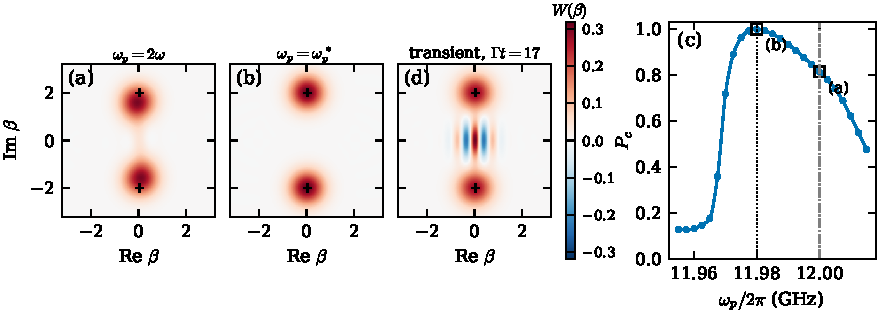
\includegraphics[width=0.95\textwidth]{figuras/apendice_fig2_estados.pdf}
\caption{Funciones de Wigner del oscilador (qubit trazado) en el esquema de Ma et al. (a) Estado estacionario con $\omega_p=2\omega$: amplitud reducida ($\alpha_{\rm eff}^2\simeq-2.5$) y peso fuera del código. (b) Estado estacionario con $\omega_p=\wps$: dos lóbulos en $\pm2i$ sin franjas, porque en el estado estacionario la paridad ya decayó. (d) Transitorio en $\Gamma t=17$, con franjas de interferencia (gato par). (c) $P_c(\omega_p)$ con los puntos de (a) y (b) marcados. Cruces: $\pm2i+g_z/\omega$. Los ejes y rótulos de las figuras están en inglés en este borrador.}
\label{fig:estados}
\end{figure}

\begin{figure}[h]
\centering
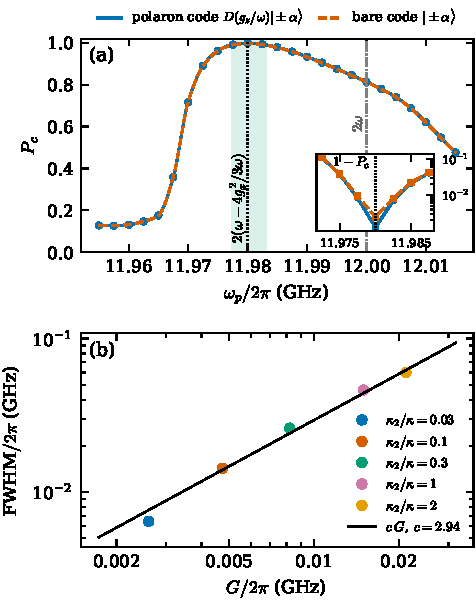
\includegraphics[width=0.62\textwidth]{figuras/fig2.pdf}
\caption{(a) $P_c$ frente a $\omega_p$ para el esquema de Ma et al.\ con el código polarónico fijo y con el código sin desplazar; la línea punteada es $2(\omega-4g_x^2/3\omega)=11.980$ y la de trazo y punto es $2\omega$. La franja es la ventana con $P_c>0.99$. Recuadro: $1-P_c$. (b) Ancho a media altura frente a $G$ para cinco valores de $\kappa_2/\kappa$, con el ajuste $\mathrm{FWHM}=cG$, $c=2.94$.}
\label{fig:fig2}
\end{figure}

\paragraph{Ancho de la resonancia.} El ancho a media altura de $P_c(\omega_p)$ escala con $G$ y no con $\kappa_2$. Con siete valores de $\kappa_2/\kappa=0.03,0.05,0.1,0.2,0.3,0.5,1$ (qubit siguiendo al drive, $\omega_q=\omega_p$, $|\alpha|^2=4$), $c=\mathrm{FWHM}/G=2.45,2.67,2.88,3.05,3.10,3.12,2.83$, es decir $c=2.87\pm0.25$; el ajuste libre da $\mathrm{FWHM}\propto\kappa_2^{0.55}=G^{1.10}$, casi lineal en $G$. En la corrida de la Fig.~\ref{fig:fig2}, con cinco valores, $c=2.93$ (media $2.92\pm0.25$). La curva es asimétrica: cae más rápido hacia $\omega_p$ menores. No se dispone de una derivación analítica de $c$.

\paragraph{Regla universal.} En la variable $x=(\omega_p-\wps)/G$ el pico cae en $|x|\leq0.09$, salvo el caso $\omega=8$, $\kappa_2/\kappa=1$, con $x=+0.16$ (la curva más asimétrica; la rejilla tiene paso $0.3$ cerca del pico). El FWHM es $2.5$--$3.25$ para $|\alpha|^2=4$ y $3.7$--$4.2$ para $|\alpha|^2=2$ (incluida la plataforma de Naseem); la asimetría crece con $\kappa_2/\kappa$: el semiancho izquierdo baja de $\sim1.3$ ($\kappa_2/\kappa=0.03$--$0.1$) a $\sim0.6$--$0.75$ ($\kappa_2/\kappa=1$--$2$) y el derecho sube a $\sim2.2$. Hay colapso del centro y una escala común de ancho, pero no un colapso total de la forma, porque el ancho depende de $|\alpha|^2$. Con $N=22$, $P_c$ en el pico va de $0.9983$ a $0.9999$ en todas las curvas salvo $\omega=6$, $g_z/\kappa=20$ ($0.9905$; $g_z/\omega=0.1$, en el límite de validez del polarón a primer orden). Convergencia: para $\omega=4$, $\kappa_2/\kappa=1$, $N=16\to22$ el pico sube $3.7\times10^{-3}$ (de $0.9945$ a $0.9983$) y el flanco en $x=1.5$ cambia $9\times10^{-5}$; con $N=16$ los máximos de las curvas con $|\alpha|^2=4$ están subestimados pero los flancos y el FWHM no se alteran.

\begin{figure}[h]
\centering
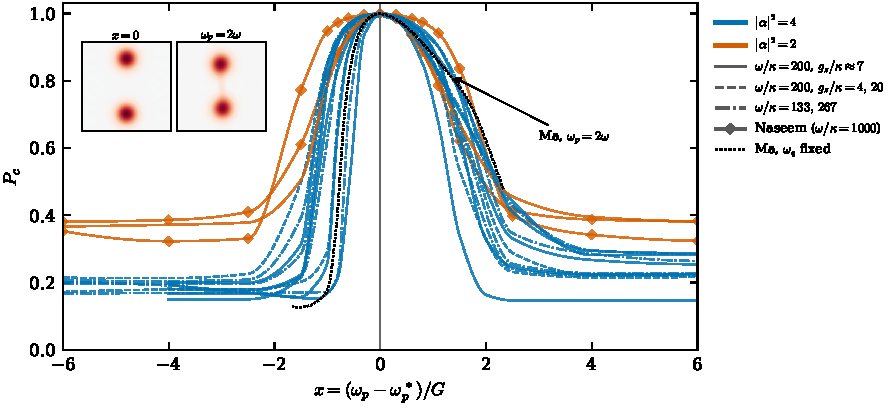
\includegraphics[width=0.95\textwidth]{figuras/apendice_resonancia_universal.pdf}
\caption{$P_c$ frente a $x=(\omega_p-\wps)/G$ para 157 estados estacionarios (curvas por $|\alpha|^2$: azul $=4$, naranja $=2$; estilos por plataforma). Todas las curvas centran su pico en $x=0$ y tienen ancho de orden $G$. Recuadro: Wigner de Ma en $x=0$ y en $\omega_p=2\omega$. Curva punteada negra: Ma con $\omega_q$ fijo.}
\label{fig:universal}
\end{figure}

\paragraph{Código polarónico.} Con el desplazamiento $d=g_z/\omega$, $1-P_c$ baja de $2.5\times10^{-3}$ a $1.3\times10^{-3}$ en la resonancia de Ma y de $5.0\times10^{-3}$ a $1.3\times10^{-3}$ en $(g_x,\omega,g_z/\kappa)=(0.05,6,12)$. Con $d=-g_z/\omega$ baja $P_c$ respecto a $d=0$, lo que confirma el signo. El desplazamiento óptimo (Nelder--Mead sobre $P_c$) es $0.03451$ en Ma, un $2.4\%$ menor que $g_z/\omega=0.03536$; la diferencia de $P_c$ entre ambos es $\leq10^{-6}$, así que se usa $d=g_z/\omega$ analítico. La caída de $P_c$ al aumentar $g_z$ era casi toda un efecto de base: la deficiencia escala como $(g_z/\omega)^2$.

\paragraph{Veredicto de la verificación independiente (V2)} (marco de laboratorio, propagador de un período): confirma $P_c=0.81180$ ($\omega_p=12$) y $0.99754$ ($\omega_p=11.98$), y un máximo del barrido en $11.9799\pm0.0005$ que coincide con la predicción $11.9800$.

\subsection{Phase-flip y figura de mérito}
\label{sec:res_pf}

La tasa de la paridad del modelo completo se extrajo por ajuste $A\,e^{-kt}+c$ sobre la serie estroboscópica con $P_c>0.99$ (verificación V3) y por el método espectral (V4, V4b). Con los parámetros de Ma ($\kappa/\omega=0.005$) el término $\kappa^2/4$ de las Ecs.~\eqref{eq:k1} cambia la predicción en $6\times10^{-6}$ y no discrimina entre las dos formas.

\begin{table}[h]
\centering
\begin{tabular}{lccc}
\toprule
medida (Ma, $\wps$) & tasa medida & predicción & razón\\
\midrule
ajuste logarítmico $\Gamma t\in[26,152]$ & $3.307\times10^{-4}$ & $3.333\times10^{-4}$ (sin $+1$, $|\alpha|^2=4$) & 0.992\\
ajuste con piso, $\Gamma t\in[26,300]$ & $3.332\times10^{-4}$ & $3.333\times10^{-4}$ (sin $+1$) & 1.000\\
ajuste con piso, con $+1$ y $|\ave{a^2}|=3.973$ & $3.332\times10^{-4}$ & $3.394\times10^{-4}$ & 0.982\\
\bottomrule
\end{tabular}
\caption{Tasa de phase-flip de Ma en la resonancia (V3). La ventana de $\Gamma t$ del ajuste logarítmico de la primera fila es la del trabajo original. El piso de paridad es $c=(6.4\pm0.6)\times10^{-4}$. El acuerdo de $1.000$ con la fórmula sin el $+1$ era una compensación de errores: el $+1$ agrega $2.5\%$ y el régimen saturado de Ma ($\kappa_2/\kappa=1$) resta $\sim2\%$.}
\label{tab:V3}
\end{table}

El ajuste logarítmico simple depende de la ventana: la razón baja de $0.992$ a $0.866$ si la ventana llega a tiempos tardíos, por el piso estacionario. Con el piso incluido la razón es $1.000$ en todas las ventanas. El origen físico del piso no se identificó; la explicación plausible es la población fuera del código (componentes vestidas y excitación residual del qubit), no verificada.

Para aislar el término $+1$ se calculó $\gamma_{\rm pf}$ espectral en $(g_x,\omega,g_z/\kappa)=(0.05,6,4)$ con $|\alpha|^2_{\rm nom}=2$, $4$ y $6$ ($N=22,22,26$), comparando con $2|\alpha|^2\kappa_1$ (A) y con la Ec.~\eqref{eq:gpf} (B), ambas con $|\alpha|^2=|\ave{a^2}|$ medido:

\begin{table}[h]
\centering
\begin{tabular}{ccccc}
\toprule
$|\alpha|^2_{\rm nom}$ & $|\ave{a^2}|$ & A ($|\ave{a^2}|$) & B ($|\ave{a^2}|$) & corrección prevista $1/(10|\alpha|^2)$\\
\midrule
2 & 1.9945 & 1.0486 & 0.9986 & $+5.0\%$\\
4 & 3.9819 & 1.0222 & 0.9971 & $+2.5\%$\\
6 & 5.9607 & 1.0128 & 0.9961 & $+1.7\%$\\
\bottomrule
\end{tabular}
\caption{Razón medido/predicho de $\gamma_{\rm pf}$ (V4b). Con $|\alpha|^2=6$ y $N=26\to32$ la tasa cambia $2\times10^{-5}$. El exceso de A sigue la forma $1/(10|\alpha|^2)$ que predice B, que se sostiene al $0.4\%$. El residuo de B ($-0.1\%$ a $-0.4\%$) crece ligeramente con $|\alpha|^2$ y no se investigó.}
\label{tab:V4b}
\end{table}

El exceso de $+1.6\%$ que se observaba a $g_z/\kappa$ pequeño con la forma A es el término $\Gamma_1^{+}(|\alpha|^2+1)$. En los puntos saturados, la caída de la razón A (hasta $0.947$ con $\kappa_2/\kappa=1$) se debe casi por completo a que el gato real es más pequeño que el nominal ($|\ave{a^2}|=3.78$ en lugar de $4$): con el $|\ave{a^2}|$ medido, A pasa a $1.003$ y B a $0.977$.

\label{sec:res_merito}

La Tabla~\ref{tab:V4} reúne 10 puntos del modelo completo con $\omega\in\{4,5,6,7\}$, $g_x\in\{0.03,\dots,0.15\}$ y $g_z/\kappa\in\{4,\dots,12\}$, todos con $N=22$, en el marco de laboratorio con $\omega_q=\omega_p=\wps$, $|\alpha|^2_{\rm nom}=4$ y $\kappa=0.03$. La tasa del modo de paridad es espectral, $\kappa_1=\gamma_{\rm pf}/(2|\alpha|^2)$ (forma A) y con la Ec.~\eqref{eq:gpf} (forma B, con $|\ave{a^2}|$).

\begin{table}[h]
\centering
\begin{tabular}{ccccccc}
\toprule
$g_x$ & $\omega$ & $g_z/\kappa$ & $\kappa_2/\kappa$ & $P_c$ est. & razón A & razón B\\
\midrule
0.03 & 6 & 4 & 0.006 & 0.99954 & 1.018 & 0.998\\
0.05 & 5 & 4 & 0.026 & 0.99932 & 1.015 & 0.996\\
0.1 & 7 & 4 & 0.052 & 0.99958 & 1.018 & 0.996\\
0.15 & 6 & 4 & 0.160 & 0.99909 & 1.016 & 0.990\\
0.05 & 6 & 5 & 0.028 & 0.99929 & 1.014 & 0.996\\
0.12 & 7 & 7 & 0.230 & 0.99890 & 1.009 & 0.993\\
0.05 & 7 & 10 & 0.082 & 0.99779 & 0.998 & 0.992\\
0.08 & 5 & 10 & 0.410 & 0.99498 & 0.973 & 0.984\\
0.1 & 4 & 10 & 1.000 & 0.99095 & 0.947 & 0.977\\
0.05 & 6 & 12 & 0.160 & 0.99504 & 0.975 & 0.986\\
\bottomrule
\end{tabular}
\caption{Verificación de la Ec.~\eqref{eq:merito} (V4, V4b). Razón A: $(\kappa_1/\kappa_2)_{\rm medido}/[(5/72)(\kappa/g_z)^2]$ con $|\alpha|^2=4$ nominal. Razón B: $\gamma_{\rm pf}$ medido entre la Ec.~\eqref{eq:gpf} con $|\alpha|^2=|\ave{a^2}|$. A $g_z/\kappa=4$ fijo, con $g_x\in\{0.03,0.05,0.1,0.15\}$ y $\omega\in\{5,6,7\}$, la razón A está en $1.015$--$1.018$ (dispersión $0.3\%$): la fórmula captura la dependencia en $g_x$ y $\omega$. Convergencia en $(0.05,6,12)$, $N=22\to28$: $r_{\rm par}$ cambia $10^{-5}$ y $P_c$ menos de $10^{-5}$.}
\label{tab:V4}
\end{table}

La independencia de $g_x$ y $\omega$ se sostiene al $0.3\%$. La razón depende de $\kappa_2/\kappa$: las fórmulas de las Ecs.~\eqref{eq:k2} y \eqref{eq:k1} son de orden dominante, exactas cuando $\kappa_2/\kappa\to0$, y el déficit medido/predicho es la primera corrección no adiabática, $\lesssim0.4\%$ para $\kappa_2/\kappa\lesssim0.05$, $\sim1\%$ en $0.2$ y $\sim2\%$ en $1$. Correlaciona con $\kappa_2/\kappa$ ($r=0.89$) más que con $P_e$ ($r=0.69$): a igual $\kappa_2/\kappa=0.16$, $P_e=3\times10^{-4}$ y $3\times10^{-3}$ dan déficits de $1.3\%$ y $1.0\%$. No hay una explicación analítica de esta corrección.

\begin{figure}[h]
\centering
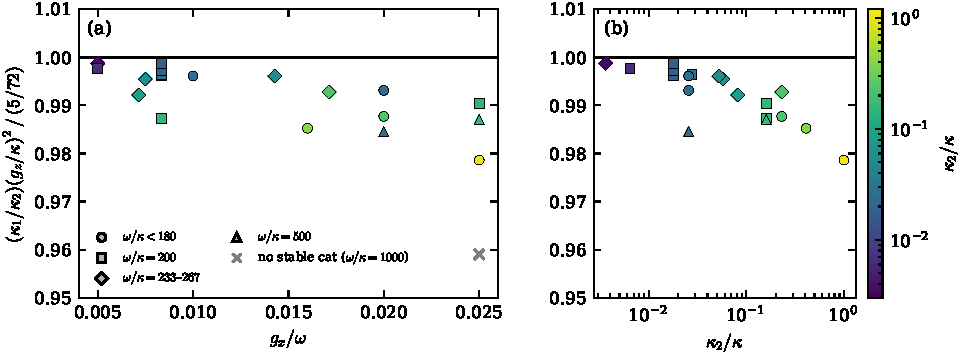
\includegraphics[width=0.95\textwidth]{figuras/principal_fig2.pdf}
\caption{Universalidad de la figura de mérito. Cociente $(\kappa_1/\kappa_2)(g_z/\kappa)^2/(5/72)$ para 19 puntos con gato estable del modelo completo, frente a (a) $g_x/\omega$ y (b) $\kappa_2/\kappa$. El color indica $\kappa_2/\kappa$ y el marcador $\omega/\kappa$. La cruz gris ($\omega/\kappa=1000$) es un punto donde el gato no se estabiliza. El rango es $0.979$--$0.999$; el déficit crece con $\kappa_2/\kappa$.}
\label{fig:universal_merito}
\end{figure}

\begin{figure}[h]
\centering
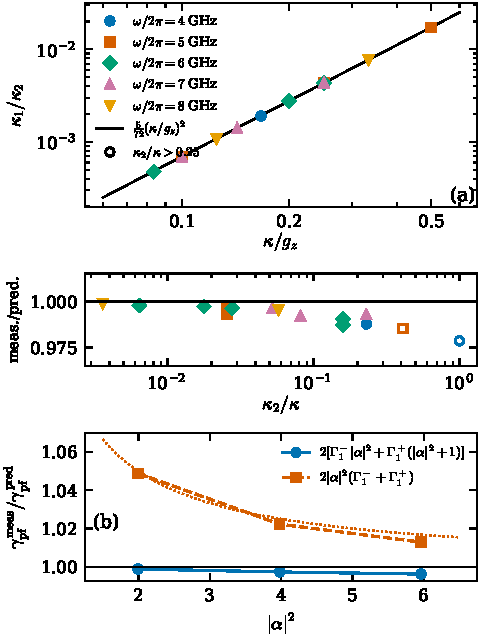
\includegraphics[width=0.62\textwidth]{figuras/fig3.pdf}
\caption{(a) $\kappa_1/\kappa_2$ frente a $\kappa/g_z$ para 15 puntos con $\omega/2\pi$ entre 4 y 8~GHz; símbolo hueco si $\kappa_2/\kappa>0.25$. Subpanel: cociente medido/predicho frente a $\kappa_2/\kappa$. (b) Cociente de la tasa de phase-flip medida y predicha frente a $|\alpha|^2$, con la Ec.~\eqref{eq:gpf} (círculos) y sin el $+1$ (cuadrados); la línea punteada es $1+1/(10|\alpha|^2)$.}
\label{fig:fig3}
\end{figure}

\subsection{Baño filtrado}
\label{sec:res_filtro}

Se usa el esquema de Ma con $\omega_q=\omega_p=\wps$, $|\alpha|^2=2$, filtro a $2\omega$ con $4J^2/\kappa_f=\kappa$ y acoplamiento en onda rotante (válido porque $J\leq0.09\ll\omega_f$). Los canales de un fonón se aislaron con el liouvilliano estático sin drive y $g_z=0$ (con $g_z\neq0$ y sin drive el intercambio de pares, resonante, mezcla $\kappa_2$ con la relajación de población). La relajación de población del oscilador es $\Gamma_1^{-}-\Gamma_1^{+}$ y la ocupación estacionaria, menos el $n$ virtual del fundamental exacto de $H$ ($1.39\times10^{-4}$), da $\Gamma_1^{+}=(\Gamma_1^{-}-\Gamma_1^{+})(\bar n-n_{\rm virt})$.

\begin{table}[h]
\centering
\begin{tabular}{cccccc}
\toprule
baño & $N$ & $N_f$ & $\Gamma_1^{-}$ medido/predicho & $\Gamma_1^{+}$ medido/predicho & $\kappa_1$ razón\\
\midrule
plano & 8 & -- & 1.0004 & 0.9995 & 1.0003\\
plano & 12 & -- & 1.0004 & 0.9994 & 1.0003\\
$\kappa_f=1$ & 8 & 2, 3 & 0.9980 & 1.0011 & 0.9981\\
$\kappa_f=0.3$ & 8 & 2, 3 & 0.9977 & 1.0011 & 0.9978\\
$\kappa_f=0.3$ & 12 & 3 & 0.9977 & 1.0011 & 0.9978\\
\bottomrule
\end{tabular}
\caption{Canales de un fonón con filtro (V5, método estático, $g_z=0$). Predicciones con $\kappa_{\rm eff}(\omega)$ y $\kappa_{\rm eff}(3\omega)$, Ec.~\eqref{eq:keff}. Los dos canales se confirman por separado al $0.2\%$, incluida la ganancia filtrada por $\kappa_{\rm eff}(3\omega)$. El filtro de dos niveles y el armónico ($N_f=3$) coinciden a $10^{-6}$; $N=8$ y $12$ coinciden.}
\label{tab:V5}
\end{table}

Con drive, la mejora de $\gamma_{\rm pf}$ respecto del baño plano coincide con la predicción que incluye el $+1$:

\begin{table}[h]
\centering
\begin{tabular}{ccccc}
\toprule
$\kappa_f$ & mejora medida & predicha con Ec.~\eqref{eq:gpf} & medido/predicho & predicha con $\kappa_1$ solo\\
\midrule
3 & 19.5 & 19.5 & 1.00 & 18.6\\
1 & 166.5 & 166.1 & 1.003 & 159.1\\
0.3 & 1838 & 1833 & 1.003 & 1757\\
0.1 & $1.65\times10^{4}$ & $1.65\times10^{4}$ & 1.003 & --\\
\bottomrule
\end{tabular}
\caption{Factor de mejora de $\gamma_{\rm pf}$ con $|\alpha|^2=2$ (unidades $2\pi\cdot$GHz, $\omega=6$). La mejora medida coincide con la predicción corregida al $0.3\%$. Comparar con $\kappa_1=\Gamma_1^{-}+\Gamma_1^{+}$ subestima la mejora un $4\%$, exactamente el efecto del $+1$: el filtro elimina casi todo $\Gamma_1^{+}$, que en el baño plano aportaba el término $\Gamma_1^{+}(|\alpha|^2+1)$ ($\Gamma_1^{+}/\Gamma_1^{-}$ baja de $0.11$ a $0.012$).}
\label{tab:mejora}
\end{table}

\paragraph{Costo en confinamiento.} Se mide con la tasa dinámica (Sección~\ref{sec:conf}) para no depender del quinto modo espectral, que es espurio en el baño plano ($|\mathrm{Im}\,\lambda|$ crece con $N$: $0.040$, $0.054$ y $0.061$ para $N=16,22,28$, y la tasa cambia un $2.2\%$ entre $N=16$ y $22$). En el baño plano la tasa dinámica es $6.98\times10^{-3}$ y $7.13\times10^{-3}$ desde los dos estados iniciales, idéntica para $N=22$ y $28$. Relativa al plano, es $0.965$ ($\kappa_f=3$), $0.967$ ($1$), $0.90$ ($0.3$) y $0.53$ ($0.1$). Convergencia con filtro ($\kappa_f=1$, $N=16\to18$; $N=20$ no cabe en memoria): $\gamma_{\rm pf}$ cambia $-1.5\times10^{-4}$ y el confinamiento $0.2$--$0.5\%$. Con $\kappa_f=0.3$--$1$ se obtiene casi toda la mejora perdiendo menos del $10\%$ de confinamiento.

\begin{figure}[h]
\centering
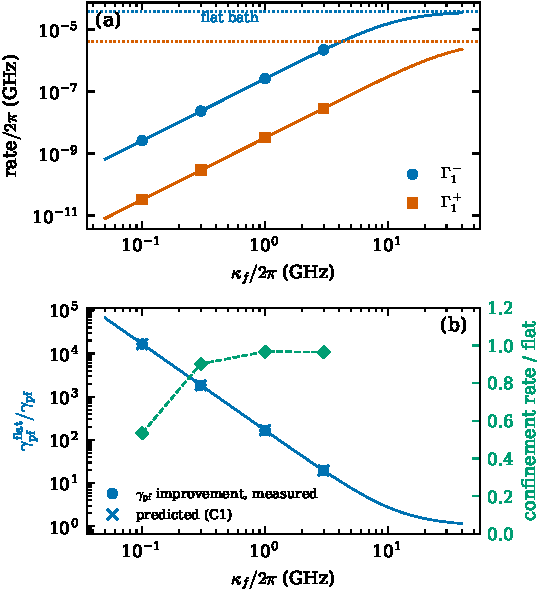
\includegraphics[width=0.62\textwidth]{figuras/fig4.pdf}
\caption{(a) Tasas de un fonón, $\Gamma_1^{-}$ y $\Gamma_1^{+}$, frente a $\kappa_f$: puntos medidos y curvas de la Ec.~\eqref{eq:keff}; líneas punteadas: baño plano. (b) Mejora de $\gamma_{\rm pf}$ respecto del baño plano (medida y predicha con la Ec.~\eqref{eq:gpf}, eje izquierdo) y tasa de confinamiento relativa al plano (eje derecho).}
\label{fig:filtro}
\end{figure}

\subsection{Confinamiento y mapa de diseño}
\label{sec:res_conf}

\paragraph{Brecha exacta con $\alpha=0$.} La Ec.~\eqref{eq:brecha} se contrastó con diagonalización densa del liouvilliano estático ($N=20$ y $26$, $\kappa=1$), contando exactamente cuatro autovalores nulos (el espacio oscuro $\{\ket{0},\ket{1}\}\otimes\ket{g}$, poblaciones y coherencias).

\begin{table}[h]
\centering
\begin{tabular}{cccc}
\toprule
$\Gamma_2/\kappa$ & $\Delta$ numérico ($N=20$) & $\Delta$ predicho & dif.\ relativa\\
\midrule
0.005 & $5.05102572\times10^{-3}$ & $5.05102572\times10^{-3}$ & $-2\times10^{-13}$\\
0.02 & $2.08712153\times10^{-2}$ & $2.08712153\times10^{-2}$ & $-8\times10^{-14}$\\
0.05 & $5.63508327\times10^{-2}$ & $5.63508327\times10^{-2}$ & $-6\times10^{-14}$\\
0.10 & 0.138196601 & 0.138196601 & $-4\times10^{-14}$\\
0.12 & 0.200000000 & 0.200000000 & $-3\times10^{-14}$\\
0.125 (punto excepcional) & 0.249999976 & 0.25 & $-9.5\times10^{-8}$\\
0.13 a 5.0 (8 valores) & 0.25 & 0.25 & $\leq2\times10^{-13}$\\
\bottomrule
\end{tabular}
\caption{Brecha del modelo mínimo con $\alpha=0$ (V6): 18 valores de $\Gamma_2/\kappa$ entre $0.005$ y $5$. Convergencia $N=20\to26$: $\leq4\times10^{-13}$, salvo en el punto excepcional ($2\times10^{-8}$). En el punto excepcional el error numérico escala como $\sqrt{\varepsilon_{\rm maq}}$, lo que explica el $10^{-7}$. Por encima del umbral los modos lentos pasan a ser oscilantes ($\mathrm{Im}\,\lambda\neq0$).}
\label{tab:V6}
\end{table}

\paragraph{Confinamiento con $|\alpha|^2=4$.} La tasa dinámica se calculó con descomposición espectral completa del liouvilliano estático del modelo mínimo (30 valores de $\kappa_2/\kappa$ entre $10^{-3}$ y $10$, $N=24$). Coincide con la espectral al $10^{-3}$ hasta $\kappa_2/\kappa\simeq0.2$. En 8 valores con $N=24,30,36$ es estable ($\leq2\times10^{-4}$), mientras que la espectral no converge en el régimen saturado ($0.216\to0.231\to0.238$ en $\kappa_2/\kappa=0.57$, la rama interior).

\begin{table}[h]
\centering
\begin{tabular}{cccc}
\toprule
$\kappa_2/\kappa$ & $\Delta/\kappa$ (dinámica) & $\Delta/\kappa_2$ & $\kappa_2^{\rm eff}/\kappa_2$\\
\midrule
$1.0\times10^{-3}$ & 0.00407 & 4.07 & 0.983\\
$1.0\times10^{-2}$ & 0.0347 & 3.46 & 0.837\\
$4.5\times10^{-2}$ & 0.0945 & 2.09 & 0.505\\
0.161 & 0.161 & 1.00 & 0.241\\
0.574 & 0.237 & 0.414 & 0.100\\
1.08 & 0.259 & 0.239 & 0.058\\
10 & 0.278 & 0.028 & 0.007\\
\bottomrule
\end{tabular}
\caption{Confinamiento dinámico del modelo mínimo con $|\alpha|^2=4$, $c=\lim\Delta/\kappa_2=4.14$ (extrapolación lineal de los tres $\kappa_2/\kappa$ menores) y $\kappa_2^{\rm eff}=\Delta/c$. La tasa satura en $\simeq0.28\kappa$ ($0.2784\kappa$ en $\kappa_2/\kappa=10$). No es un techo estricto en $\kappa/4$: el valor exacto $\kappa/4$ corresponde a $\alpha=0$ (Ec.~\eqref{eq:brecha}) y con $|\alpha|^2=4$ la meseta queda algo por encima. La saturación empieza en $\kappa_2/\kappa\simeq1/(4c)=0.060$, donde $\kappa_2^{\rm eff}/\kappa_2\simeq0.43$. En el límite $\kappa_2\to0$, $\epsilon(g_z/\kappa)^2=0.0707$ frente a $5/72=0.0694$ ($\kappa_2^{\rm eff}/\kappa_2=0.983$).}
\label{tab:conf}
\end{table}

\paragraph{Con filtro.} El costo del filtro en confinamiento se calculó con el modelo mínimo más el modo filtro, $J(\spl b+\mathrm{h.c.})$, $\kappa_f\D[b]$, $4J^2/\kappa_f=\kappa$, $N=20$, $N_f=3$, con $\kappa_f/\omega=0.05$. Cociente $\Delta_{\rm filtro}/\Delta_{\rm plano}$:

\begin{center}
\begin{tabular}{ccccccc}
\toprule
$\kappa_2/\kappa$ & $10^{-3}$ & $0.01$ & $0.03$ & $0.1$ & $0.3$ & $1$\\
\midrule
$\Delta_{\rm filtro}/\Delta_{\rm plano}$ & 1.002 & 1.014 & 1.037 & 1.051 & 0.955 & 0.480\\
\bottomrule
\end{tabular}
\end{center}

Con $\kappa_2$ pequeño el filtro confina algo más rápido (hasta $+5\%$); en saturación, la mitad. Controles: con $\kappa_f=1000\kappa$ se recupera el plano (1.0015); $N=20\to26$ cambia menos de $0.1\%$; $N_f=2\to3$ cambia $1.2\%$. Por encima de $\kappa_2/\kappa=1.5$ el retorno de $P_c(t)$ no es monótono (sobrepaso) y la tasa no está definida.

\label{sec:res_mapa}

Se compara el confinamiento del modelo completo con el del modelo mínimo. El cociente $\mathrm{conf}_{\rm completo}/\Delta_{\rm min}$ es $1.00$--$1.03$ para $g_x/\omega\lesssim0.01$, baja a $0.93$--$0.86$ para $g_x/\omega\simeq0.014$--$0.02$ y a $0.64$ para $g_x/\omega=0.025$ con $\kappa_2/\kappa=0.16$. La causa es el corrimiento $\chi\hn\Pe$ de la Ec.~\eqref{eq:chi}: el modelo efectivo estático con $\chi$ reproduce el confinamiento del modelo completo al $0.5$--$4\%$ (por ejemplo $0.632$ frente a $0.640$ en el peor punto) y el efectivo sin $\chi$ reproduce el modelo mínimo ($\geq0.99$). Con $\omega/\kappa=500$ (mismos $g_x/\omega$, $g_z/\kappa$ y $\kappa_2/\kappa$) la desviación crece a $\mathrm{conf}/\Delta_{\rm min}=0.175$ (el efectivo con $\chi$ da $0.176$) y $0.13$. Con $\omega/\kappa=1000$ ($\chi|\alpha|^2/\kappa=4.3$ y $6.7$) el gato no se estabiliza: $P_c$ estacionario $0.49$ y $0.95$, con dinámica no monótona. El umbral empírico es $\mathrm{conf}/\Delta_{\rm min}\geq0.98$ para $\chi|\alpha|^2/\kappa\lesssim0.2$, $0.91$ en $0.45$ y $0.64$ en $1.3$: la pérdida es del $5\%$ en $\chi|\alpha|^2/\kappa\simeq0.3$.

\begin{figure}[h]
\centering
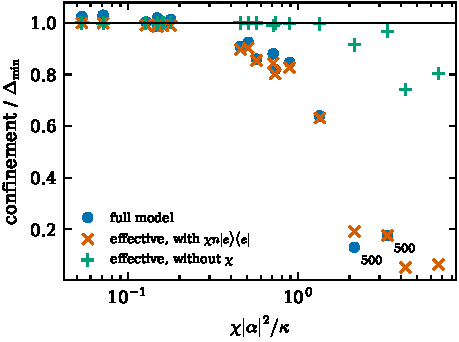
\includegraphics[width=0.62\textwidth]{figuras/p9_diagnostico.pdf}
\caption{Confinamiento del modelo completo relativo al del modelo mínimo frente a $\chi|\alpha|^2/\kappa$. Círculos: modelo completo. Cruces: efectivo con $\chi\hn\Pe$. Signos $+$: efectivo sin $\chi$. Las anotaciones ``500'' marcan los puntos con $\omega/\kappa=500$.}
\label{fig:p9}
\end{figure}

\paragraph{Mapa de diseño.} Con la Ec.~\eqref{eq:k1k} y la Tabla~\ref{tab:conf} se construye $\epsilon=\kappa_1/\kappa_2^{\rm eff}=(5/72)(\kappa/g_z)^2\,\kappa_2/\kappa_2^{\rm eff}$ en el plano $(g_z/\kappa,\kappa_2/\kappa)$, con $\kappa_2^{\rm eff}$ de la Tabla~\ref{tab:conf}. Como verificación adiabática, $\epsilon(g_z/\kappa)^2=0.0707$ en $\kappa_2/\kappa=10^{-3}$ frente a $5/72=0.0694$. El umbral $\epsilon=1/220$ se desplaza de $g_z/\kappa=3.909$ (Sección~\ref{sec:merito}) a $3.94$ en el mapa, porque en $\kappa_2/\kappa=10^{-3}$ el confinamiento efectivo es $0.983$ del nominal. Para el valor de $\omega/\kappa=200$ la frontera $\chi|\alpha|^2/\kappa=0.3$ es la Ec.~\eqref{eq:frontera}; para $\omega/\kappa=1000$, la curva correspondiente. En la Fig.~\ref{fig:mapa} se superponen los 15 puntos del modelo completo ($N=22$): $\epsilon_{\rm completo}/\epsilon_{\rm mapa}$ va de $0.97$ a $1.55$, y las mayores desviaciones están del lado de $\chi|\alpha|^2/\kappa$ grande, donde el mapa sobreestima el confinamiento en más del $5\%$. Ma tiene $\chi|\alpha|^2/\kappa=2.7$: fuera de la región cuantitativa del mapa, aunque su gato se estabiliza ($P_c=0.9987$). Naseem tiene $0.19$ (con $|\alpha|^2=2$): dentro.

\begin{figure}[h]
\centering
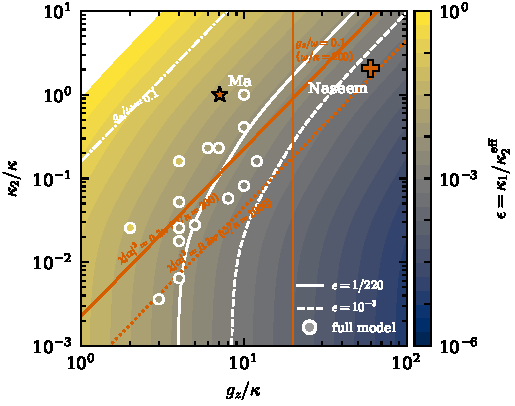
\includegraphics[width=0.75\textwidth]{figuras/principal_fig3.pdf}
\caption{Mapa de diseño con baño plano. Color: $\epsilon=\kappa_1/\kappa_2^{\rm eff}$ para $|\alpha|^2=4$. Contorno blanco continuo: $\epsilon=1/220$; discontinuo: $\epsilon=10^{-3}$. Curvas naranjas: $\chi|\alpha|^2/\kappa=0.3$ para $\omega/\kappa=200$ (continua) y $1000$ (punteada); vertical: $g_z/\omega=0.1$ para $\omega/\kappa=200$. Línea blanca de trazo y punto: $g_x/\omega=0.1$. Círculos: 15 puntos del modelo completo ($N=22$). Estrella: Ma. Cruz: Naseem (con $\omega/\kappa=1000$, en la zona sombreada calculada con $\omega/\kappa=200$; con su $\omega/\kappa$ real $g_z/\omega=0.06<0.1$).}
\label{fig:mapa}
\end{figure}

\paragraph{Mapa con baño filtrado y piso intrínseco.} La figura central compara el mapa plano con el filtrado ($\kappa_f/\omega=0.05$, es decir $\kappa_f/\kappa=10$ con $\omega/\kappa=200$), con el costo del filtro en confinamiento incluido. En el régimen adiabático el umbral en $g_z/\kappa$ pasa de $3.94$ (plano) a $0.094$ (filtro), un factor $0.0238$. La predicción de la Sección~\ref{sec:filtro} es $\sqrt{f/(10/9)}=0.0239$, con $f=6.32\times10^{-4}$ y $\kappa_f/2\omega=0.025$. El factor se mantiene en $0.023$--$0.024$ hasta $\kappa_2/\kappa\simeq0.3$ y sube a $0.034$ en $\kappa_2/\kappa=1$, donde el filtro frena el confinamiento.

\paragraph{Verificación del modelo completo con filtro.} ($N_f=2$, $\omega/\kappa=200$, $\kappa_f=0.3$.)
\begin{center}
\begin{tabular}{ccccc}
\toprule
$(\kappa_2/\kappa,g_z/\kappa)$ & cantidad & $N=16$ & $N=20$ & $N=22$\\
\midrule
$(0.03,12)$ & $\gamma_{\rm pf}$/predicho & 2.880 & 0.986 & 0.978\\
$(0.03,12)$ & $\epsilon_{\rm completo}/\epsilon_{\rm mapa}$ & 2.831 & 0.987 & 0.979\\
$(0.3,12)$ & $\gamma_{\rm pf}$/predicho & 2.261 & 0.980 & 0.977\\
$(0.3,12)$ & $\epsilon_{\rm completo}/\epsilon_{\rm mapa}$ & 2.288 & 0.975 & 0.972\\
\bottomrule
\end{tabular}
\end{center}
El exceso con $N=16$ ($\times2.3$--$2.9$) es un artefacto de truncamiento: con $|\alpha|^2=4$, polarón $g_z/\omega=0.06$ y filtro, $N=16$ no está convergido. Con $N=20\to22$, $\gamma_{\rm pf}$ cambia $0.8\%$ y $0.3\%$, y el confinamiento menos de $0.05\%$. La precisión declarada con filtro es de $2$--$3\%$. En $(0.03,4)$ ($N=16$) $\epsilon_{\rm completo}/\epsilon_{\rm mapa}=1.03$. Validaciones con $N=22$: $|\mathrm{Tr}\rho-1|=0$ y mínimo autovalor $\geq-5.6\times10^{-9}$.

\paragraph{Piso intrínseco.} Con $\kappa_1\to\kappa_1^{\rm filt}+\gamma$, la Sección~\ref{sec:merito} da $\kappa_2^{\rm eff}/\kappa\geq220\gamma/\kappa$. El piso depende solo de $\gamma/\kappa=(\omega/\kappa)/Q$. Ma ($Q=10^7$, $\omega/\kappa=200$) tiene $\gamma/\kappa=2\times10^{-5}$; Naseem ($\gamma/2\pi=15$~Hz, $\kappa/2\pi=100$~kHz) tiene $1.5\times10^{-4}$. Con $\gamma/\kappa=2\times10^{-4}$, $\epsilon=1/220$ solo se alcanza en la franja $\kappa_2/\kappa\simeq0.19$--$0.33$ y $\epsilon=10^{-3}$ no se alcanza; dentro de la zona verificada ($\chi|\alpha|^2\leq0.3\kappa$, $\omega/\kappa=200$) solo queda $g_z/\kappa\gtrsim9.3$ ($\kappa_2/\kappa=0.19$) a $11.9$ ($0.32$), es decir $g_z/\kappa\gtrsim10$. Con $\gamma/\kappa=2\times10^{-5}$ el umbral $1/220$ se desplaza $+44\%$ en $\kappa_2/\kappa=0.01$, $+14\%$ en $0.03$, $+7\%$ en $0.1$, $+5\%$ en $0.3$ y $+8\%$ en $1$; el piso nunca baja del $10\%$ de $\kappa_1^{\rm filt}$. Verificación con el modelo completo con filtro y $\gamma=2\times10^{-4}\kappa$ como $\gamma\D[a]$, $N=22$:
\begin{itemize}
\item $(\kappa_2/\kappa,g_z/\kappa)=(0.25,14)$, $\chi|\alpha|^2/\kappa=0.17$: $\gamma_{\rm pf}$/predicho $=1.007$, confinamiento/mapa $=0.979$, $\epsilon_{\rm completo}/\epsilon_{\rm mapa}=1.028$ y $\epsilon_{\rm completo}=4.39\times10^{-3}<1/220$. El diseño de la franja verificada funciona.
\item $(0.25,6)$, $\chi|\alpha|^2/\kappa=0.93$, fuera de la zona ($N=20$): $\gamma_{\rm pf}$/predicho $=1.000$ pero confinamiento/mapa $=0.751$ y $\epsilon_{\rm completo}/\epsilon_{\rm mapa}=1.33$. La frontera de $\chi$ vale con filtro, con una pérdida coherente con la Fig.~\ref{fig:p9} ($0.91$ en $0.45$, $0.64$ en $1.3$).
\end{itemize}

\begin{figure}[h]
\centering
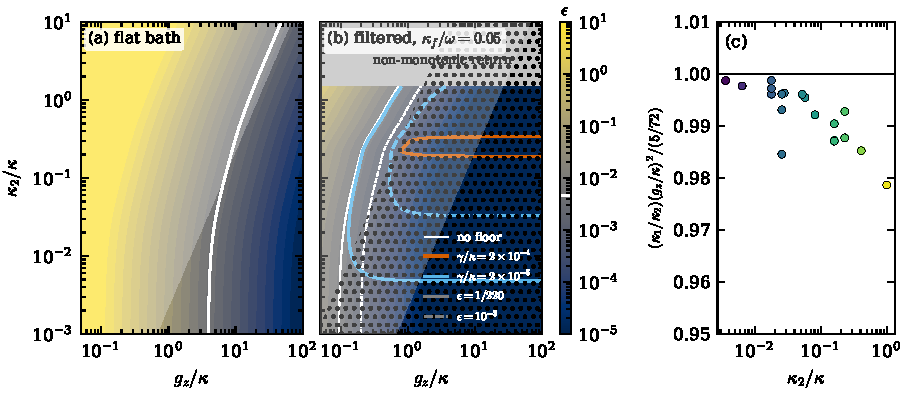
\includegraphics[width=0.98\textwidth]{figuras/figura_central_sinpiso.pdf}
\caption{Mapa de diseño (a) con baño plano y (b) con baño filtrado ($\kappa_f/\omega=0.05$), para $|\alpha|^2=4$ y $\omega/\kappa=200$. El color muestra $\epsilon$ sin pérdida intrínseca; las curvas incluyen $\gamma/\kappa=2\times10^{-5}$ (celeste) y $2\times10^{-4}$ (naranja), continuas para $\epsilon=1/220$ y discontinuas para $\epsilon=10^{-3}$; la línea blanca fina es el caso sin piso. La región punteada es $\chi|\alpha|^2>0.3\kappa$. La zona gris ($\kappa_2/\kappa>1.5$) es donde el retorno de $P_c$ no es monótono. (c) Colapso del modelo completo: $(\kappa_1/\kappa_2)(g_z/\kappa)^2/(5/72)$ frente a $\kappa_2/\kappa$ (19 puntos con gato estable).}
\label{fig:central}
\end{figure}

\subsection{Sesgo térmico}
\label{sec:res_term}

El estudio térmico usa el modelo efectivo estático con el qubit (P9) y el filtro explícitos ($N_f=2$), con baños térmicos (Ec.~\eqref{eq:ME_T}) y $N=22$ ($N=24$ en la isla). Espectro con \texttt{eigs} disperso (shift-invert). La isla es $\kappa_2/\kappa=0.25$, $g_z/\kappa=14$, $\omega/\kappa=200$, $|\alpha|^2=4$, con $\kappa_f/\omega=0.05$ o baño plano. Las rejillas son $x\in[1,25]$ (40 valores) $\times$ $\kappa_2/\kappa\in[0.02,0.4]$ con $g_z/\kappa=14$ ($\chi|\alpha|^2/\kappa\leq0.27$) y $\times$ $\gamma/\kappa\in[10^{-6},10^{-3}]$ en la isla. El eje superior de la figura es $f_q$ a $10$~mK, $x\cdot208.37$~MHz.

Los niveles de referencia $\eta=100$ y $\eta=220$ son convenciones: $\eta=100$ es el criterio de sesgo que se usó en el trabajo de validación del esquema de Naseem y no tiene una justificación propia en este proyecto; $220$ es el umbral de Guillaud y Mirrahimi, que se define sobre $\kappa_2/\kappa_1$ y no sobre $\gamma_{\rm pf}/\gamma_{\rm bf}$.

\begin{table}[h]
\centering
\begin{tabular}{ccccc}
\toprule
baño & $\gamma/\kappa$ & $x^{*}(\eta=100)$ & $x^{*}(\eta=220)$ & $f_q$ a 10~mK ($\eta=100$/$220$)\\
\midrule
filtrado & $2\times10^{-5}$ & 10.11 & 10.91 & 2.11 / 2.27 GHz\\
filtrado & $2\times10^{-4}$ & 7.78 & 8.59 & 1.62 / 1.79 GHz\\
plano & $2\times10^{-5}$ & 8.19 & 9.01 & 1.71 / 1.88 GHz\\
plano & $2\times10^{-4}$ & 7.18 & 8.00 & 1.50 / 1.67 GHz\\
\bottomrule
\end{tabular}
\caption{Umbrales de $x=hf_q/k_BT$ en la isla ($N=22$). $N=22\to24$ cambia $x^{*}$ en $\leq0.008$. La diferencia local relativa de $\eta$ junto a cada umbral es $\leq1.5\%$.}
\label{tab:term}
\end{table}

El filtro sube el requisito en $x$ porque reduce $\gamma_{\rm pf}$ (el numerador de $\eta$), mientras que $\gamma_{\rm bf}/n_q$ solo sube un $28\%$ ($0.032\kappa\to0.041\kappa$ en la isla). $\eta$ mide sesgo, no calidad. El umbral depende de $\gamma/\kappa$ mientras $\gamma$ domine $\gamma_{\rm pf}$; con $\gamma/\kappa\lesssim10^{-5}$ en el plano se vuelve casi independiente de $\gamma$ ($x^{*}(100)\simeq8.4$, régimen térmico puro); con filtro sigue moviéndose. Como control, si $\Gamma_1^{-}$ usa $n(\omega)$ y $\Gamma_1^{+}$ usa $n(3\omega)$ (las frecuencias reales del fonón), con filtro $\gamma_{\rm pf}$ cambia $\leq10^{-4}$ y $x^{*}(100)$ no cambia ($10.114$); en el plano $\gamma_{\rm pf}$ sube $+1.1\%$ en $x=10$ y $+2.9\%$ en $x=8$, y $x^{*}(100)$ pasa de $8.197$ a $8.173$ ($-0.3\%$).

\paragraph{Bit-flip térmico.} El ajuste directo de $\gamma_{\rm bf}-\gamma_{\rm bf}(T\to0)=c_{\rm bf}n_q\kappa$ con $n_q\in[10^{-5},10^{-2}]$ da un exponente local $p=1.00$--$1.02$ y
\begin{center}
\begin{tabular}{ccccc}
\toprule
$\kappa_2/\kappa$ & 0.02 & 0.05 & 0.2 & 0.4\\
\midrule
$c_{\rm bf}$ con filtro & $2.62\times10^{-4}$ & $1.65\times10^{-3}$ & $2.75\times10^{-2}$ & $8.42\times10^{-2}$\\
$c_{\rm bf}$ en el plano & $2.76\times10^{-4}$ & $1.67\times10^{-3}$ & $2.23\times10^{-2}$ & $6.20\times10^{-2}$\\
\bottomrule
\end{tabular}
\end{center}
con incertidumbre (semirrango intercuartil) $\leq2\%$. Se ajusta $c_{\rm bf}\propto(G/\kappa)^s$ con $G/\kappa=\sqrt{\kappa_2/\kappa}/2$: $s=3.96\pm0.04$ con filtro y $s=3.69\pm0.05$ en el plano. Por tanto, $\gamma_{\rm bf}\simeq0.05\,n_q\kappa$ como constante, que se usó en el trabajo de validación de Naseem, no es una ley: $c_{\rm bf}$ varía más de dos órdenes de magnitud con $\kappa_2/\kappa$. La supresión con $|\alpha|^2$ ($x=9$ y $12$, $|\alpha|^2=2$--$6$) es $d\ln\gamma_{\rm bf}/d|\alpha|^2\simeq-0.55$ y $-0.64$ en el plano y $-0.43$ y $-0.42$ con filtro; en el plano coincide con el buffer de dos niveles de Gautier et al.~\cite{Gautier2022} para $g_2/\kappa\simeq0.3$ ($\simeq-0.55$). La supresión fuerte ($-1.0$ a $-1.4$) solo aplica con $g_2/\kappa\lesssim0.1$.

\begin{figure}[h]
\centering
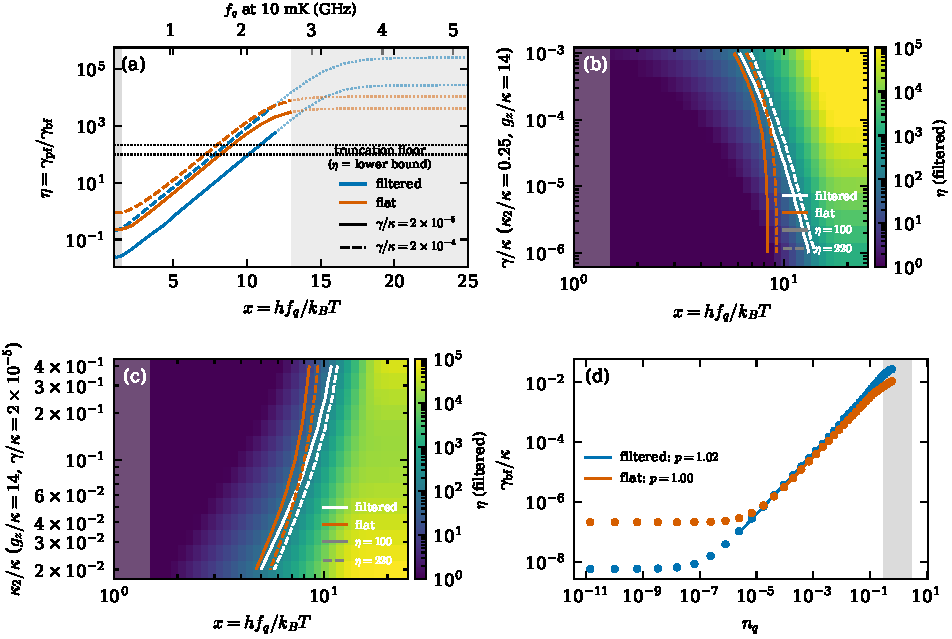
\includegraphics[width=0.98\textwidth]{figuras/figura_termica.pdf}
\caption{(a) $\eta=\gamma_{\rm pf}/\gamma_{\rm bf}$ frente a $x=hf_q/k_BT$ en la isla, con filtro (azul) y baño plano (naranja), para $\gamma/\kappa=2\times10^{-5}$ (continua) y $2\times10^{-4}$ (discontinua). Más allá de $x=13$ las curvas (punteadas) son el piso de truncamiento a $T\to0$ y $\eta$ es una cota inferior. (b) Mapa de $\eta$ en $(\gamma/\kappa,x)$; (c) en $(\kappa_2/\kappa,x)$ con $\gamma/\kappa=2\times10^{-5}$. Contornos blancos: baño filtrado; naranjas: plano; continuos $\eta=100$, discontinuos $\eta=220$. (d) $\gamma_{\rm bf}/\kappa$ frente a $n_q$, con exponente local $p$.}
\label{fig:termica}
\end{figure}

\paragraph{Convergencia y validaciones.} En la isla, 34 de 160 puntos cambian más del $3\%$ entre $N=22$ y $24$, todos con $x\gtrsim13$ (piso de $T=0$); ningún umbral cae ahí. La región caliente $n_q>0.3$ ($x<1.47$) se excluye. Hermiticidad antes de hermitizar (sin simetrizar por paridad): $\|\rho-\rho^{\dagger}\|\leq1.4\times10^{-11}$; $|\mathrm{Tr}\rho-1|\leq6.7\times10^{-16}$; mínimo autovalor $\geq-8.7\times10^{-17}$. La validación con el modelo completo (filtro y temperatura, $N=22$) está abierta; véase la Sección~\ref{sec:limites}.

\subsection{Plataformas, literatura y limitaciones abiertas}
\label{sec:res_plat}

\begin{table}[h]
\centering
\begin{tabular}{lccc}
\toprule
 & Ma et al. & Naseem & Liu et al.\\
\midrule
$\kappa/\omega$ & 0.005 & 0.001 & 0.90\\
$g_z/\kappa$ & 7.1 & 60 & 0.22\\
$\kappa_2/\kappa$ & 1.0 & 2.07 & 0.031\\
$\kappa_1/\kappa_2$ & $1.4\times10^{-3}$ & $9.2\times10^{-5}$ & fuera de validez\\
$\chi|\alpha|^2/\kappa$ & 2.7 & 0.19 & --\\
$\gamma/\kappa$ & $2\times10^{-5}$ ($Q=10^7$, sin verificar) & $1.5\times10^{-4}$ & --\\
$hf_q/k_BT$ (10 mK) & 58 & 0.96 ($f_q=200$~MHz) & --\\
veredicto & confinamiento saturado; fuera de la frontera de $\chi$ & falla térmica (no calculada con $\kappa_2/\kappa=2.07$) & fuera del régimen perturbativo\\
\bottomrule
\end{tabular}
\caption{Posición de las plataformas. Tabla provisional, por rehacer con $\kappa_1/\kappa_2^{\rm eff}$ y $x$ a 10~mK para todas las columnas.}
\label{tab:plat}
\end{table}

\paragraph{Liu et al.} Con $\kappa/\omega=0.9$ y $g_z/\omega=0.2$ la jerarquía $\kappa\ll\omega$ no se cumple y ninguna fórmula de la Sección~\ref{sec:deriv} aplica. La integración de su Ec.~(9) completa (convención con $2\varepsilon_p\cos(\omega_pt)\tilde\sigma_x$, que reproduce su Ec.~(11) y el $\alpha=1.58$ de su Fig.~2) no forma el gato: $F\leq0.35$ frente a $0.95$ del efectivo, $|\ave{a^2}|$ máximo $0.4$--$1.1$ (analítico $1.25$ o $2.5$), y la fórmula de la paridad falla en $95$--$99\%$. Convergencia $N=20\to28$ $\leq2\times10^{-3}$; validaciones cumplidas ($|\mathrm{Tr}\rho-1|\leq4.4\times10^{-16}$, $\|\rho-\rho^{\dagger}\|\leq1.3\times10^{-15}$, autovalores $\geq-1.5\times10^{-10}$). Se interpreta como que la eliminación adiabática no vale en ese régimen. Es una conclusión numérica propia, pendiente de contrastar con los autores; adicionalmente, la Ec.~(9) con $\varepsilon_p\cos(\omega_pt)\tilde\sigma_x$ da por onda rotante $\varepsilon_p/2$ ($\alpha^2=1.25$), por lo que el coeficiente del coseno debería ser $2\varepsilon_p$ para ser coherente con la Ec.~(11): posible inconsistencia interna, inferida y no verificada contra su derivación.

\paragraph{Resumen de las correcciones a la literatura.}
\begin{itemize}
\item Ma et al., Ec.~(4): omite $-(g_x^2/\omega)\hn$ (el corrimiento del oscilador con el qubit en $\ket{g}$, total $-4g_x^2/3\omega$) y da $3g_x^2/\omega$ para el corrimiento del qubit (el correcto es $4g_x^2/3\omega$). El término de pares es correcto. Consecuencia: resonancia en $11.98$, no en $12$.
\item Liu et al., Ec.~(11): omite $-(4g_x^2/3\omega)\hn$. Coeficiente de pares correcto.
\item Naseem: su código no incluye $\delta_1$ en el hamiltoniano efectivo; su Ec.~(11) usa $g_{\rm eff}=g$ en lugar de $2g$; su recomendación de aumentar $\kappa$ contradice $\kappa_1/\kappa_2\propto\kappa^2$. La relación $g_{\rm eff}=2g$ se confirmó por dos métodos: la medición directa de la oscilación de Rabi de dos fotones sin disipación (coincide con $2\sqrt2\cdot(2g)$ a menos del $5\%$) y el álgebra exacta de la transformación polarónica (que reproduce el coeficiente $-2g$ de su Ec.~(9) y no el $+g$ de su Ec.~(11)).
\item Ma y Liu atribuyen a su esquema la conservación de la paridad en el estado estacionario. El modelo completo no la conserva: el estado estacionario es una mezcla de $\ket{\pm\alpha}$ y la tasa de phase-flip está dada por la Ec.~\eqref{eq:gpf}. Hou et al.\ no se incluye en la comparación cuantitativa porque no se ha leído su artículo.
\end{itemize}

\label{sec:limites}

\begin{enumerate}
\item Validación térmica con el modelo completo. En $(\kappa_2/\kappa,g_z/\kappa)=(0.25,14)$, $x=10.1$, $N=22$, el modelo completo en el laboratorio da $\gamma_{\rm pf}=1.56\times10^{-4}$, plausible frente al efectivo, pero no reproduce un modo lento de pozo: el modo con $\lambda\simeq-1$ decae a $\simeq4\times10^{-2}$ ($N=12$) y $7\times10^{-2}$ ($N=22$), frente a $\gamma_{\rm bf}\simeq10^{-6}$ del efectivo. La selección del modo se corrigió y la discrepancia persiste. El diagnóstico a $T=0$, con y sin $\gamma$, está en curso. Hasta resolverlo, los umbrales térmicos de la Tabla~\ref{tab:term} no están validados con el modelo completo. La hermiticidad cruda de esa corrida fue $2.7\times10^{-10}$, por encima de la tolerancia.
\item Déficit no adiabático de $1$--$2\%$ en las fórmulas de orden dominante (Sección~\ref{sec:res_merito}): sin explicación analítica.
\item Validez del mapa. Solo está verificado en la isla ($\kappa_2/\kappa\simeq0.19$--$0.33$, $g_z/\kappa\gtrsim10$, $\gamma/\kappa=2\times10^{-4}$) y con $\chi|\alpha|^2\leq0.3\kappa$. No se debe generalizar fuera de ella.
\item Tasa de confinamiento con $\alpha\neq0$. Solo se conoce numéricamente. La tasa espectral no converge en el régimen saturado; la relevante es la dinámica.
\item Punto de Naseem térmico con $\kappa_2/\kappa=2.07$: no calculado. La tabla de plataformas es provisional.
\item Resultados retirados durante el trabajo y que no deben usarse: la brecha con máximo en $\Gamma_2/\kappa\simeq0.13$ y la rama de Floquet con $|\mathrm{Im}\,\lambda|\propto N$ (artefactos de modos de borde de Fock); el ``techo $\kappa/4$'' con $|\alpha|^2\neq0$; el $\gamma_{\rm bf}\simeq0.05\,n_q\kappa$ como constante; el exceso $\times2.9$ de $\gamma_{\rm pf}$ con $N=16$; el uso de $\alpha_{\rm eff}$ para definir el código en $P_c$.
\item Revisión de citas y lectura de Hou et al.\ pendientes; revisión humana independiente de las derivaciones.
\end{enumerate}

\bibliographystyle{unsrt}
\bibliography{refs_informe}
\end{document}
